%
% The first command in your LaTeX source must be the \documentclass command.
%\documentclass[acmsmall,screen=true,authorversion=true,nonacm=true]{acmart}
\documentclass[acmsmall]{acmart}
%
% for preprint:
% \documentclass[manuscript]{acmart}
%
% for camera-ready:
% \documentclass[acmsmall]{acmart}
%
%

\usepackage{tikz}
\usepackage[usenames,dvipsnames]{pstricks}
\usepackage{epsfig}

%\usepackage{palatino}
\RequirePackage{ifthen}
\RequirePackage{amsmath}
\RequirePackage{amssymb}
\RequirePackage{listings}
\RequirePackage{mathrsfs}
\RequirePackage{xspace}
\RequirePackage{graphics}

% PACKAGES FOR ORGANIZING THE STRUCTE OF DOCUMENT
%\usepackage{minipage}
\usepackage{latexsym}
\usepackage{multicol}
\usepackage{multirow}
\usepackage{lscape}  % Useful for wide tables or figures.
\usepackage{xspace}
\usepackage{paralist}
%\usepackage{framed}
%\usepackage{lipsum}
% DEFINING THE BOUNDARY --- DONE IN DOCUMENT.
%\usepackage[left=1.25in,right=1.25in,top=1in,bottom=1.25in]{geometry}

%%% SECTION TITLE APPEARANCE
% \usepackage{sectsty}
% \allsectionsfont{\sffamily\mdseries\upshape} % (See the fntguide.pdf for font help)
% (This matches ConTeXt defaults)

%%% HEADERS & FOOTERS
% \usepackage{fancyhdr} % This should be set AFTER setting up the page geometry
% \pagestyle{fancy} % options: empty , plain , fancy
% \renewcommand{\headrulewidth}{0pt} % customise the layout...
% \lhead{}\chead{}\rhead{}
% \lfoot{}\cfoot{\thepage}\rfoot{}


% PACKAGES FOR FIGURES
\usepackage{xcolor}
\usepackage{float}
\usepackage{subfigure}
%\usepackage{subfloat}
\usepackage{graphicx}
\usepackage{caption}
\usepackage{wrapfig}
%\usepackage{pifont}
%\usepackage{subcaption}
%\usepackage{subfigure}  % for subfigures
%\usepackage{setspace}
%\usepackage[justification=raggedright]{caption}	% makes captions ragged right - thanks to Bryce Lobdell

%AMS AND OTHER MISC PACKAGES
\usepackage{keyval}
\usepackage{amsmath,amssymb,amsfonts,url,listings,mathrsfs}
%reference
\usepackage{hyperref}
%\usepackage[pdftex,colorlinks,citecolor=webblue,linkcolor=webblue,urlcolor=webblue]{hyperref}

%ALGORITHM PACKAGE
%\usepackage{algorithm,algorithmic}
%
%\usepackage[pdftex,colorlinks,citecolor=webblue,linkcolor=webred,backref,pagebackref]{hyperref}
%\usepackage[linesnumbered,lined,commentsnumbered]{algorithm2e}
%\usepackage[linesnumbered,boxed,lined,commentsnumbered,algochapter]{algorithm2e}


%DEFINITIONS FOR MARKING CHANGES AND COMMENTS
\newcommand{\authcomment}[1]{\textbf{[[#1]]}}
%\newcommand{\sayan}[1]{\textcolor{blue}{[[#1]]}}
%\newcommand{\sridhar}[1]{\textcolor{red}{[[#1]]}}
\newcommand{\sridhar}[1]{\textcolor{brown}{[[#1]]}}
\newcommand{\stan}[1]{\textcolor{blue}{[[#1]]}}

% DEFINING COLORS
\definecolor{reddish}{rgb}{1,.8,0.8}
\definecolor{blueish}{rgb}{0.8,.8,1}
\definecolor{greenish}{rgb}{.8,1,0.8}
\definecolor{yellowish}{rgb}{1,1,.20}
\definecolor{webred}{rgb}{0.5,0,0}
\definecolor{webblue}{rgb}{0,0,0.8}

% DEFINITIONS FOR TEXT FORMATTING
\newcommand{\figuresize}{\scriptsize}
\newcommand{\equationsize}{\footnotesize}

% ADHOC DEFINITIONS FOR EACH AND EVERY PAPER
\newcommand{\trajmet}{discrepancy function\/}
\newcommand{\TrajMet}{Trajectory Metric}
\newcommand{\RT}{{\em reachtubes}}
\newcommand{\hylaa}{{HyLAA}}
\newcommand{\valsim}{{\sf valSim}}
\newcommand{\tool}{C2E2 \/}
\newcommand{\fulltoolname}{\textbf{C}heck \textbf{E}xecute \textbf{C}ompare \textbf{E}ngine}
\newcommand{\leftshift}[2]{\relax\ifmmode (#1 \lhd #2) \else $(#1 \lhd #2)$ \fi}
\newcommand{\mayInt}{\relax\ifmmode \mathit{mayInt} \else $\mathit{mayInt}$ \fi}
\newcommand{\mustInt}{\relax\ifmmode \mathit{mustInt} \else $\mathit{mustInt}$ \fi}
\newcommand{\notInt}{\relax\ifmmode \mathit{notInt} \else $\mathit{notInt}$ \fi}
\newcommand{\alarm}{\relax\ifmmode \mathit{Alert} \else $\mathit{Alert}$ \fi}
\newcommand{\unsafe}{\relax\ifmmode \mathit{Unsafe} \else $\mathit{Unsafe}$ \fi}
\newcommand{\xsep}{\relax\ifmmode \mathit{xsep} \else $\mathit{xsep}$\fi}
\newcommand{\ysep}{\relax\ifmmode \mathit{ysep} \else $\mathit{ysep}$ \fi}
\newcommand{\etime}{{\sf time}}
\newcommand{\ub}{{\sf ub}}
\newcommand{\lb}{{\sf lb}}
\newcommand{\emode}{{\sf mode}}
\newcommand{\erange}{{\sf range}}
\newcommand{\fbls} {functionally bounded linear span}
\newcommand{\fblsupper} {Functionally bounded linear span}

% COMMANDS USED IN DEFINITIONS
\newcommand{\meansl}{[\![}
\newcommand{\meansr}{]\!]}
\newcommand{\means}[1]{\meansl #1 \meansr}
\newcommand{\Nset}[1]{[[#1]]}

% ROUTINELY USED COMMANDS
\newcommand{\refinement}[1]{\relax\ifmmode \mathit{refine}(#1) \else $\mathit{refine}(#1)$ \fi}
\newcommand{\diff}{{\sf diff}}
\newcommand{\diameter} {\mathsf{diameter}}
\newcommand{\cntr} {\mathsf{center}}
\newcommand{\ball}[1] {B_{#1}}
\newcommand{\true}{\relax\ifmmode \mathit true \else \em true \/\fi}
\newcommand{\false}{\relax\ifmmode \mathit false \else \em false \/\fi}
% \newcommand{\lnot}{\neg} % Already defined
% \newcommand{\land}{\wedge} % Already defined
% \newcommand{\lor}{\vee} % Already defined
\newcommand{\limplies}{\Rightarrow}
\newcommand{\liff}{\Leftrightarrow}
%\newcommand{\T}{\mathit{true}}
%\newcommand{\F}{\mathit{false}}
% \newcommand{\to}{\relax\ifmmode \rightarrow \else $\rightarrow$\fi} % Already defined
\newcommand{\fro}{\relax\ifmmode \leftarrow \else $\leftarrow$\fi}


% COMMANDS FOR MATH SPECIFIC ITEMS
\newcommand{\nnt}{{\sf T}^{\geq 0}}             %nonnegative time points
\newcommand{\post}{{\sf T}^{>0}}                %positive time points
\newcommand{\Variables}{{\sf V}}                %variables

\newcommand{\num}[1]{\relax\ifmmode \mathbb #1\else $\mathbb #1$\fi}
\newcommand{\nnnum}[1]{\relax\ifmmode 
  {\mathbb #1}_{\geq 0} \else ${\mathbb #1}_{\geq 0}$
  \fi}
\newcommand{\npnum}[1]{\relax\ifmmode 
  {\mathbb #1}_{\leq 0} \else ${\mathbb #1}_{\leq 0}$
  \fi}
\newcommand{\pnum}[1]{\relax\ifmmode 
  {\mathbb #1}_{> 0} \else ${\mathbb #1}_{> 0}$
  \fi}
\newcommand{\nnum}[1]{\relax\ifmmode 
  {\mathbb #1}_{< 0} \else ${\mathbb #1}_{< 0}$
  \fi}
\newcommand{\plnum}[1]{\relax\ifmmode 
  {\mathbb #1}_{+} \else ${\mathbb #1}_{+}$
  \fi}
\newcommand{\nenum}[1]{\relax\ifmmode 
  {\mathbb #1}_{-} \else ${\mathbb #1}_{-}$
  \fi}

\newcommand{\reals}{{\num R}}                    %reals
\newcommand{\nnreals}{{\nnnum R}}                    %nonnegative reals
\newcommand{\realsinfty}{{\num R} \cup \{\infty, -\infty\}}                    %nonnegative reals
\newcommand{\plreals}{{\plnum R}}                    %positive reals
\newcommand{\naturals}{{\num N}}                      %natural numbers
\newcommand{\integers}{{\num Z}}                      %integers
\newcommand{\rationals}{{\num Q}}                      %rationals
\newcommand{\nnrationals}{{\nnnum Q}}                   % nonnegative rationals
\newcommand{\Time}{{\num T}}  
\newcommand{\bools}{{\num B}}  
\newcommand{\plintegers}{{\plnum Z}}                      %integers
\newcommand{\deq}{\mathrel{\stackrel{\scriptscriptstyle\Delta}{=}}}
\newcommand{\intervals}{\relax \ifmmode \mathbb{IR} \else $\mathbb{IR}$ \fi}
\newcommand{\nnintervals}{\relax \ifmmode \mathbb{IR}^{+} \else $\mathbb{IR}^{+}$ \fi}
%\setlength{\mathindent}{0pt}

% COMMANDS FOR LABELS
\renewcommand{\eqref}[1]{Equation~(\ref{eq:#1})}
\newcommand{\eqlabel}[1]{\label{eq:#1}}
\newcommand{\figref}[1]{Figure~\ref{fig:#1}}
\newcommand{\figrefs}[2]{Figures~\ref{fig:#1} and~\ref{fig:#2}}
\newcommand{\figlabel}[1]{\label{fig:#1}}
\newcommand{\tabref}[1]{Table~\ref{table:#1}}
\newcommand{\tablabel}[1]{\label{table:#1}}
\newcommand{\defref}[1]{Definition~\ref{def:#1}}
\newcommand{\deflabel}[1]{\label{def:#1}}
\newcommand{\exref}[1]{Example~\ref{exmp:#1}}
\newcommand{\exlabel}[1]{\label{exmp:#1}}
\newcommand{\scref}[1]{Section~\ref{sec:#1}}
\newcommand{\secreftwo}[2]{Sections~\ref{sec:#1}~and~\ref{sec:#2}}
\newcommand{\sclabel}[1]{\label{sec:#1}}
\newcommand{\applabel}[1]{\label{app:#1}}
\newcommand{\appref}[1]{Appendix~\ref{app:#1}}
\newcommand{\lnlabel}[1]{\label{line:#1}}
\newcommand{\lnrngref}[2]{lines~\ref{line:#1}--\ref{line:#2}\xspace}
\newcommand{\lnref}[1]{line~\ref{line:#1}\xspace}
\newcommand{\thmref}[1]{Theorem~\ref{thm:#1}\xspace}
%\newcommand{\seclabel}[1]{\label{sec:#1}}
%\newcommand{\secref}[1]{Section~\ref{sec:#1}}
%\newcommand{\figlabel}[1]{\label{fig:#1}}
%\newcommand{\figref}[1]{Figure~\ref{fig:#1}}


% COMMANDS FOR SECTIONS AND ORGANIZATION

\newenvironment{noqedproof}{\pf}{}
\newcommand{\pf}{\par\noindent{\bf Proof:}~}
% \newcounter{theorem}
% \setcounter{theorem}{0}
% 
%  \newtheorem{theorem}{Theorem}
%  \newtheorem{lemma}[theorem]{Lemma}
%  \newtheorem{corollary}[theorem]{Corollary}
%  \newtheorem*{claim}{Claim}
%  \newtheorem{assumption}{Assumption}
%  \theoremstyle{definition}
%  \newtheorem{definition}{Definition}
%  \newcommand{\qed}{\hfill{\rule{2mm}{2mm}}\medskip}
%  \newenvironment{proof}{\pf}{\qed}
%  \newtheorem{proposition}[theorem]{Proposition}
% \newtheorem{inv}[theorem]{Invariant}
 
%    \newcounter{rem}
%  \setcounter{rem}{0}
%  
%   \newenvironment{remark}
%   {\refstepcounter{rem} \vspace{2ex}\par\noindent
%    \textbf{Remark}~\textbf{\therem~}}
 
% \newcounter{example}
%  \setcounter{example}{0}

%   \newtheorem{example}[example]{Example}
%  \newcounter{example}
  
%  \newenvironment{example}
%  {\refstepcounter{example} \vspace{2ex}\par\noindent
%  \textbf{Example}~\textbf{\theexample~}}%{\qed}
% \newexample{example}[example]{Example}

%\theoremstyle{remark}
%\newcounter{example}
% \newtheorem{example}{Example}[chapter]
% {\refstepcounter{theorem} \vspace{2ex}\par\noindent
% \textbf{Example}~\textbf{\theexampletheorem~}}{\qed}
 
 \def\examplenonum#1#2{
        \vspace{.15in}
        \noindent
        {\bf Example #1}{\em ~(continued)}{\bf .}
        {#2}{\qed}
        }
        
% \renewcommand{\theequation}{\thesection.\arabic{equation}}
% \renewcommand{\thefigure}{\thesection.\arabic{figure}}
% \renewcommand{\thetable}{\thesection.\arabic{table}}
% \newcommand{\Section}[1]{\section{#1}%
%    \setcounter{equation}{0}\setcounter{figure}{0}\setcounter{table}{0}%
%    \setcounter{example}{0}}


%%%%%%%%%%%%%%%%%
%%%%%%%%%%%%%%%%%
%%%%% TIOA STUFF %%%%%
%%%%%%%%%%%%%%%%%
%%%%%%%%%%%%%%%%%



% EXECUTIONS TRACES and FRAGS
\newcommand{\extb}[1]{\relax\ifmmode {\sf ExtBeh}_{#1} \else ${\sf ExtBeh}_{#1}$\fi} 
\newcommand{\tdists}[1]{\relax\ifmmode {\sf Tdists}_{#1} \else ${\sf Tdists}_{#1}$\fi} 

\newcommand{\exec}[1]{\relax\ifmmode {\sf Execs}_{#1} \else ${\sf Exec}_{#1}$\fi} 
\newcommand{\execf}[1]{\relax\ifmmode {\sf Execs}^*_{#1} \else ${\sf Exec}^*_{#1}$\fi} 
\newcommand{\execi}[1]{\relax\ifmmode {\sf Execs}^\omega_{#1} \else ${\sf Exec}^\omega_{#1}$\fi} 

\newcommand{\ctrace}[1]{\relax\ifmmode {\sf Ctraces}_{#1} \else ${\sf Ctraces}_{#1}$\fi} 

\newcommand{\trace}[1]{\relax\ifmmode {\sf Traces}_{#1} \else ${\sf Traces}_{#1}$\fi} 
\newcommand{\tracef}[1]{\relax\ifmmode {\sf Traces}^*_{#1} \else ${\sf Traces}^*_{#1}$\fi} 
\newcommand{\tracei}[1]{\relax\ifmmode {\sf Traces}^\omega_{#1} \else ${\sf Traces}^\omega_{#1}$\fi} 

\newcommand{\frag}[1]{\relax\ifmmode {\sf Frags}_{#1} \else ${\sf Frags}_{#1}$\fi} 
\newcommand{\fragf}[1]{\relax\ifmmode {\sf Frags}^*_{#1} \else ${\sf Frags}^*_{#1}$\fi} 
\newcommand{\fragi}[1]{\relax\ifmmode {\sf Frags}^\omega_{#1} \else ${\sf Frags}^\omega_{#1}$\fi} 

\newcommand{\reach}[1]{\relax\ifmmode {\sf Reach}_{#1} \else ${\sf Reach}_{#1}$\fi} 
\newcommand{\pair}[2]{\relax\ifmmode \langle #1, #2 \rangle \else $\langle #1, #2 \rangle$\fi} 

\newcommand{\TE}{\relax\ifmmode \mathit{Time} \else $\mathit{Time}$ \fi} 
\newcommand{\EQ}{\relax\ifmmode \mathit{Enq} \else $\mathit{Enq}$ \fi} 
\newcommand{\DQ}{\relax\ifmmode \mathit{Deq} \else $\mathit{DeqTime}$ \fi} 
\newcommand{\E}{\relax\ifmmode \mathsf{E} \else $\mathsf{E}$ \fi}

\newcommand{\loc}{\relax\ifmmode \mathit{loc} \else $\mathit{loc}$ \fi}
\newcommand{\abs}{\relax\ifmmode \mathit{abs} \else $\mathit{abs}$ \fi}

\newcommand{\execs}{{\exec{}}}
\newcommand{\traces}{{\trace{}}}
\newcommand{\fragss}{{\frag{}}}
\newcommand{\fexecs}{{\execf{}}}
\newcommand{\ftraces}{{\tracef{}}}
\newcommand{\ffragss}{{\fragf{}}}
\newcommand{\iexecs}{{\execi{}}}
\newcommand{\itraces}{{\tracei{}}}
\newcommand{\ifragss}{{\fragi{}}}
\newcommand{\fstate}{{\sf fstate}}  
\newcommand{\lstate}{{\sf lstate}}  
\newcommand{\ltime}{{\sf ltime}}  
\newcommand{\dur}{{\sf dur}}  
\newcommand{\mode}{{\sf mode}}  
\newcommand{\ftime}{{\sf ftime}}  

% 
% \newenvironment{anotation}[1][Nancy]{\begin{quote}\small[[[#1]]]}{\normalsize\end{quote}}
% \newcommand{\ba}{\begin{anotation}}
% \newcommand{\ea}{\end{anotation}}
% 
% \newcommand{\bcb}{\chgbarbegin}
% \newcommand{\ecb}{\chgbarend}
% \chgbarwidth 1pt
% 
% \newcommand{\dec}{\ensuremath{{:}}}
% \newcommand{\eqdef}{\mathbin{::=}}
% \newcommand{\I}{{\ensuremath{\cap}}}



% OPERATIONS ON SETS, RELATIONS AND FUNCTIONS
\newcommand{\pow}[1]{{\bf P}(#1)} % powerset
\newcommand{\inverse}[1]{#1^{-1}}
\newcommand{\range}[1]{\ms{range{(#1)}}}
\newcommand{\domain}[1]{{\it dom}(#1)}
\newcommand{\type}[1]{\ms{type{(#1)}}}
\newcommand{\dtype}[1]{\ms{dtype{(#1)}}} % dynamic type
\newcommand{\restr}{\mathrel{\lceil}}
\newcommand{\proj}{\matrel{\lceil}}
\newcommand{\restrrange}{\mathrel{\downarrow}}
\newcommand{\point}[1]{\wp(#1)}                 %point trajectory



% HYBRID AUTOMATA
\def\A{{\cal A}} % HA
\def\B{{\cal B}} % HA
\def\C{{\cal C}} % HA
\def\D{{\cal D}} % set of discrete steps
\def\E{{\cal E}} % HA
\def\F{{\cal F}} % HA
\def\G{{\cal G}} % pieces of SHIOA
\def\H{{\cal H}} % HA
\def\I{{\cal I}} % environment sequence
\def\K{{\cal K}} % environment sequence
\def\L{{\cal L}} % environment sequence
\def\M{{\cal M}} % Mode switching transitions
\def\O{{\cal O}} % outcome function
\def\P{{\cal P}} % set of modes
\def\Q{{\cal Q}} % set of modes
\def\R{{\cal R}} % relation
\def\S{{\cal S}} % set of trajectories
\def\T{{\cal T}} % set of trajectories
\def\V{{\cal V}} % Lyapunov function
\def\U{{\cal U}} % set of trajectories
\def\X{{\cal X}} % Lyapunov function
\def\Y{{\cal Y}} % set of trajectories
\def\Z{{\cal Z}} % set of trajectories

\def\u{{\mathsf u}} % set of inputs

% more special characters

\newcommand{\col}[1]{\relax\ifmmode \mathscr #1\else $\mathscr #1$\fi}
\def\statemodels{\col{S}}


% Names of actions, automata etc
\definecolor{HIOAcolor}{rgb}{0.776,0.22,0.07}
\newcommand{\HIOA}{\textcolor{HIOAcolor}{\tt HIOA\hspace{3pt}}}
\newcommand{\PVS}{\textcolor{HIOAcolor}{\tt PVS\hspace{3pt}}}
\newcommand{\PVSnogap}{\textcolor{HIOAcolor}{\tt PVS\hspace{1pt}}}
\newcommand{\HIOAbiggap}{\textcolor{HIOAcolor}{\tt HIOA\hspace{6pt}}}
\newcommand{\HIOAnogap}{\textcolor{HIOAcolor}{\tt HIOA}}
\newcommand{\anyrelation}{\lessgtr}

% Transformation for ADT
\newcommand{\SC}[2]{\relax\ifmmode {\tt Scount}(#1,#2) \else ${\tt Scount}(#1,#2)$\fi} 
\newcommand{\SCM}[2]{\relax\ifmmode {\tt Smin}(#1,#2) \else ${\tt Smin}(#1,#2)$\fi} 
\newcommand{\Aut}[1]{\relax\ifmmode {\tt Aut}(#1) \else ${\tt Aut}(#1)$\fi} 

\newcommand{\auto}[1]{{\operatorname{\mathsf{#1}}}}
\newcommand{\act}[1]{{\operatorname{\mathsf{#1}}}}
\newcommand{\smodel}[1]{{\operatorname{\mathsf{#1}}}}
\newcommand{\pvstheory}[1]{{\operatorname{\mathit{#1}}}}
%\newcommand{\auto}[1]{\relax\ifmmode \sf #1\else $\sf #1$\fi}
%\newcommand{\act}[1]{\relax\ifmmode \sf #1\else $\sf #1$\fi}


\newcommand{\Automaton}{{\bf automaton}}
\newcommand{\Asserts}{{\bf asserts}}
\newcommand{\Assumes}{{\bf assumes}}
\newcommand{\Backward}{{\bf backward}}
\newcommand{\By}{{\bf by}}
\newcommand{\Case}{{\bf case}}
\newcommand{\Choose}{{\bf  choose}}
\newcommand{\Components}{{\bf components}}
\newcommand{\Const}{{\bf const}}
\newcommand{\Converts}{{\bf converts}}
\newcommand{\Do}{{\bf do}}
\newcommand{\Eff}{{\bf eff}}
\newcommand{\Else}{{\bf else}}
\newcommand{\Elseif}{{\bf elseif}}
\newcommand{\Enumeration}{{\bf enumeration}}
\newcommand{\Ensuring}{{\bf ensuring}}
\newcommand{\Exempting}{{\bf exempting}}
\newcommand{\Fi}{{\bf fi}}
\newcommand{\For}{{\bf for}}
\newcommand{\Forward}{{\bf forward}}
\newcommand{\Freely}{{\bf freely}}
\newcommand{\From}{{\bf from}}
\newcommand{\Generated}{{\bf generated}}
\newcommand{\Local}{{\bf local}}
\newcommand{\Hidden}{{\bf hidden}}
\newcommand{\If}{{\bf if}}
\newcommand{\In}{{\bf in}}
\newcommand{\Implies}{{\bf implies}}
\newcommand{\Includes}{{\bf includes}}
\newcommand{\Introduces}{{\bf introduces}}
\newcommand{\Input}{{\bf input}}
\newcommand{\Kind}{{\bf kind}}
\newcommand{\Initially}{{\bf initially}}
\newcommand{\Internal}{{\bf internal}}
\newcommand{\Invariant}{{\bf invariant}}
\newcommand{\Od}{{\bf od}}
\newcommand{\Of}{{\bf of}}
\newcommand{\Output}{{\bf output}}
\newcommand{\Partitioned}{{\bf partitioned}}
\newcommand{\Pre}{{\bf pre}}
\newcommand{\Signature}{{\bf signature}}
\newcommand{\Simulation}{{\bf simulation}}
\newcommand{\Sort}{{\bf sort}}
\newcommand{\States}{{\bf states}}
\newcommand{\Tasks}{{\bf tasks}}
\newcommand{\Then}{{\bf then}}
\newcommand{\To}{{\bf to}}
\newcommand{\Trait}{{\bf trait}}
\newcommand{\Traits}{{\bf traits}}
\newcommand{\Transitions}{{\bf transitions}}
\newcommand{\Tuple}{{\bf tuple}}
\newcommand{\Type}{{\bf type}}
\newcommand{\Union}{{\bf union}}
\newcommand{\Uses}{{\bf uses}}
\newcommand{\Where}{{\bf where}}
\newcommand{\While}{{\bf while}}
\newcommand{\With}{{\bf with}}

% Spacing
\newcommand{\FFF}{\vspace{0.1in}}
\newcommand{\BBB}{\hspace{-0.1in}}


%% defs FROM ptioa PAPER

\newcommand{\remove}[1]{}
\newcommand{\salg}[1]{\relax\ifmmode {\mathcal F}_{#1}\else ${\mathcal F}_{#1}$\fi} 
\newcommand{\msp}[1]{\relax\ifmmode (#1, \salg{#1}) \else $(#1, \salg{#1})$\fi} 
\newcommand{\msprod}[2]{\relax\ifmmode ( #1 \times #2, \salg{#1} \otimes \salg{#2}) \else $(#1 \times #2, \salg{#1} \otimes \salg{#2})$\fi} 
\newcommand{\dist}[1]{\relax\ifmmode {\mathcal P}\msp{#1}
  \else ${\mathcal P}\msp{#1}$\fi} 
\newcommand{\subdist}[1]{\relax\ifmmode {\mathcal S}{\mathcal P}\msp{#1} 
  \else ${\mathcal S}{\mathcal P}\msp{#1}$\fi} 
\newcommand{\disc}[1]{\relax\ifmmode {\sf Disc}(#1)
  \else ${\sf Disc}(#1)$\fi} 

\newcommand{\Trajeq}{\relax\ifmmode {\mathcal R}_\T \else ${\mathcal R}_\T$\fi} 
\newcommand{\Acteq}{\relax\ifmmode {\mathcal R}_A \else ${\mathcal R}_A$\fi} 
\newcommand{\noop}{\relax\ifmmode \lambda \else $\lambda$\fi} 
\newcommand{\close}[1]{\relax\ifmmode \overline{#1} \else $\overline{#1}$\fi} 

\newcommand{\corrtasks}{\mathop{\mathsf {c}}}
\newcommand{\full}{\mathop{\mathsf {full}}}
%\newcommand{\fstate}{\mathop{\mathsf {fstate}}}
%\newcommand{\lstate}{\mathop{\mathsf {lstate}}}
\newcommand{\tdist}{\mathop{\mathsf {tdist}}}
\newcommand{\extbeh}{\mathop{\mathsf {extbeh}}}
%\newcommand{\apply}{\mathop{\mathsf {apply}}}
\newcommand{\apply}[2]{\mathop{\mathsf {apply}({#1},{#2})}}
%\newcommand{\applytwo}{\mathop{\mathsf {apply2}}}
\newcommand{\support}{\mathop{\mathsf {supp}}}
\newcommand{\maxrng}{\mathop{\mathsf {max}}}
\newcommand{\relation}{\mathrel{R}}
\newcommand{\cone}{C}
%\newcommand{\tracef}{\mathord{\mathsf {trace}}}
\newcommand{\flatten}{\mathord{\mathsf {flatten}}}
\newcommand{\discrete}{\mathord{\mathsf {Disc}}}
\newcommand{\lift}[1]{\mathrel{{\mathcal L}(#1)}}
\newcommand{\expansion}[1]{\mathrel{{\mathcal E}(#1)}}
%End of commands added by Roberto on May, 12

%>> Ling, December 2005

\newcommand{\subdisc}{\operatorname{\mathsf {SubDisc}}}
\newcommand{\tran}{\operatorname{\mathsf {tran}}}
%\newcommand{\act}{\operatorname{\mathsf {act}}}

\renewcommand{\execs}{{\operatorname{\mathsf {Execs}}}}
\newcommand{\frags}{{\operatorname{\mathsf {Frags}}}}

\newcommand{\tracefnc}{{\operatorname{\mathsf {trace}}}}

\newcommand{\finite}{{\operatorname{\mathsf {finite}}}}
\newcommand{\hide}{{\operatorname{\mathsf {hide}}}}

\newcommand{\early}{{\operatorname{\mathsf {Early}}}}
\newcommand{\late}{{\operatorname{\mathsf {Late}}}}
\newcommand{\toss}{{\operatorname{\mathsf {Toss}}}}

\newcommand{\define}{:=}

\newcommand{\pc}{{\operatorname{\mathsf {counter}}}}
\newcommand{\chosen}{{\operatorname{\mathsf {chosen}}}}

\newcommand{\rand}{{\operatorname{\mathsf {random}}}}
\newcommand{\unif}{{\operatorname{\mathsf {unif}}}}

\newcommand{\ie}{i.e.,\xspace}
\newcommand{\Ie}{I.e.,\xspace}

\newcommand{\eg}{e.g.,\xspace}
\newcommand{\Eg}{E.g.,\xspace}

% IOA related stuff

\newcommand{\mybox}[3]{
  \framebox[#1][l]
  {
    \parbox{#2}
    {
      #3
    }
  }
}

\newcommand{\two}[4]{
  \parbox{.98\columnwidth}{\vspace{1pt} \vfill
    \parbox[t]{#1\columnwidth}{#3}%
    \hspace{.5cm}
    \parbox[t]{#2\columnwidth}{#4}%
  }}

\newcommand{\twosep}[4]{
  \parbox{\columnwidth}{\vspace{1pt} \vfill
    \parbox[t]{#1\columnwidth}{#3}%
        \vrule width 0.2pt
    \parbox[t]{#2\columnwidth}{#4}%
  }}

\newcommand{\eqntwo}[4]{
  \parbox{\columnwidth}{\vspace{1pt} \vfill
    \parbox[t]{#1\columnwidth}{$ #3 $}
    \parbox[t]{#2\columnwidth}{$ #4 $}
  }}

\newcommand{\three}[6]{\vspace{1pt} \vfill
        \parbox{\columnwidth}{%
        \parbox[t]{#1\columnwidth}{#4}%
        \parbox[t]{#2\columnwidth}{#5}%
        \parbox[t]{#3\columnwidth}{#6}%
      }}


\newcommand{\lit}[1]{ \relax\ifmmode
                \mathord{\mathcode`\-="702D\sf #1\mathcode`\-="2200}
                \else {\it #1} \fi }

%\newcommand{\act}[1]{%
%  \relax\ifmmode
%                \mathord{\mathcode`\-="702D\sf #1\mathcode`\-="2200}%
%                \else
%                {\sf #1\/}%
%                \fi }

\lstdefinelanguage{ioa}{
  basicstyle=\figuresize,
  keywordstyle=\bf \figuresize,
  identifierstyle=\it \figuresize,
  emphstyle=\tt \figuresize,
  mathescape=true,
  tabsize=20,
%  tabsize=4,
  sensitive=false,
  columns=fullflexible,
  keepspaces=false,
  flexiblecolumns=true,
%  basewidth=0.5em,
  basewidth=0.05em,
  moredelim=[il][\rm]{//},
  moredelim=[is][\sf \figuresize]{!}{!},
  moredelim=[is][\bf \figuresize]{*}{*},
  keywords={automaton,and, 
         choose,const,continue, components,
         discrete, do, derived,
         eff, external,else, elseif, evolve, end,each,
         fi,for, forward, from,
         hidden,
         in,input,internal,if,invariant, initially, imports,
     let,
     or, output, operators, od, of,
     pre, prob,
     return,
     such,satisfies, stop, signature, simulation, state, stochastic,
     trajectories,trajdef, transitions, that,then, type, types, to, tasks,
     variables, vocabulary, uni,
     when,where, with,while},
  emph={set, seq, tuple, map, array, enumeration},   
   literate=
        {(}{{$($}}1
        {)}{{$)$}}1
        % LaTeX math symbols
        {\\in}{{$\in\ $}}1
        {\\preceq}{{$\preceq\ $}}1
        {\\subset}{{$\subset\ $}}1
        {\\subseteq}{{$\subseteq\ $}}1
        {\\supset}{{$\supset\ $}}1
        {\\supseteq}{{$\supseteq\ $}}1
        {\\forall}{{$\forall$}}1
        {\\le}{{$\le\ $}}1
        {\\ge}{{$\ge\ $}}1
        {\\gets}{{$\gets\ $}}1
        {\\cup}{{$\cup\ $}}1
        {\\cap}{{$\cap\ $}}1
        {\\langle}{{$\langle$}}1
        {\\rangle}{{$\rangle$}}1
        {\\exists}{{$\exists\ $}}1
        {\\bot}{{$\bot$}}1
        {\\rip}{{$\rip$}}1
        {\\emptyset}{{$\emptyset$}}1
        {\\notin}{{$\notin\ $}}1
        {\\not\\exists}{{$\not\exists\ $}}1
        {\\ne}{{$\ne\ $}}1
        {\\to}{{$\to\ $}}1
        {\\implies}{{$\implies\ $}}1
        % LSL symbols (one-character)
        {<}{{$<\ $}}1
        {>}{{$>\ $}}1
        {=}{{$=\ $}}1
        {~}{{$\neg\ $}}1
        {|}{{$\mid$}}1
        {'}{{$^\prime$}}1
        % LSL symbols (two characters)
        {\\A}{{$\forall\ $}}1
        {\\E}{{$\exists\ $}}1
        {\\/}{{$\vee\,$}}1
        {\\vee}{{$\vee\,$}}1
        {/\\}{{$\wedge\,$}}1
        {\\wedge}{{$\wedge\,$}}1
        {=>}{{$\Rightarrow\ $}}1
        {->}{{$\rightarrow\ $}}1
        {<=}{{$\Leftarrow\ $}}1
        {<-}{{$\leftarrow\ $}}1
%        {<=}{{$\leq$}}1
%        {>=}{{$\geq$}}1
        {~=}{{$\neq\ $}}1
        {\\U}{{$\cup\ $}}1
        {\\I}{{$\cap\ $}}1
        {|-}{{$\vdash\ $}}1
        {-|}{{$\dashv\ $}}1
        {<<}{{$\ll\ $}}2
        {>>}{{$\gg\ $}}2
        {||}{{$\|$}}1
%%       {\[\]}{{\[\,\]}}2 {\{\}}{{\{\,\}}}2
%%        {[}{{$\langle$}}1
%%        {]}{{$\rangle$}}1
        {[}{{$[$}}1
        {]}{{$\,]$}}1
        {[[}{{$\langle$}}1
        {]]]}{{$]\rangle$}}1
        {]]}{{$\rangle$}}1
        {<=>}{{$\Leftrightarrow\ $}}2
        {<->}{{$\leftrightarrow\ $}}2
        {(+)}{{$\oplus\ $}}1
        {(-)}{{$\ominus\ $}}1
        {_i}{{$_{i}$}}1
        {_j}{{$_{j}$}}1
        {_{i,j}}{{$_{i,j}$}}3
        {_{j,i}}{{$_{j,i}$}}3
        {_0}{{$_0$}}1
        {_1}{{$_1$}}1
        {_2}{{$_2$}}1
        {_n}{{$_n$}}1
        {_p}{{$_p$}}1
        {_k}{{$_n$}}1
        {-}{{$\ms{-}$}}1
        {@}{{}}0
        {\\delta}{{$\delta$}}1
        {\\R}{{$\R$}}1
        {\\Rplus}{{$\Rplus$}}1
        {\\N}{{$\N$}}1
        {\\times}{{$\times\ $}}1
        {\\tau}{{$\tau$}}1
        {\\alpha}{{$\alpha$}}1
        {\\beta}{{$\beta$}}1
        {\\gamma}{{$\gamma$}}1
        {\\ell}{{$\ell\ $}}1
        {--}{{$-\ $}}1
        {\\TT}{{\hspace{1.5em}}}3        
      }

\lstdefinelanguage{ioaNums}[]{ioa}
{
  numbers=left,
  numberstyle=\tiny,
  stepnumber=2,
  numbersep=4pt
%  firstnumber=1
}

\lstdefinelanguage{ioaNumsRight}[]{ioa}
{
  numbers=right,
  numberstyle=\tiny,
  stepnumber=2,
  numbersep=4pt
%  firstnumber=1
}

\newcommand{\ioa}{\lstinline[language=IOA]}

\lstnewenvironment{IOA}%
  {\lstset{language=IOA}}
  {}

\lstnewenvironment{IOANums}%
  {
  \if@firstcolumn
    \lstset{language=IOA, numbers=left, firstnumber=auto}
  \else
    \lstset{language=IOA, numbers=right, firstnumber=auto}
  \fi
  }
  {}

\lstnewenvironment{IOANumsRight}%
  {
    \lstset{language=IOA, numbers=right, firstnumber=auto}
  }
  {}

%\lstnewenvironment{IOA}%
%  {\lstset{language=ioaLang}
%   \csname lst@SetFirstLabel\endcsname}
%  {\csname lst@SaveFirstLabel\endcsname\vspace{-4pt}\noindent}

\newcommand{\figioa}[5]{
  \begin{figure}[#1]
      \hrule \F
      {\figuresize \bf #2}
      \lstinputlisting[language=ioaLang]{#5}
      \F \hrule \F
      \caption{#3}
      \label{fig: #4}
  \end{figure}
}

\newcommand{\linefigioa}[9]{

}

\newcommand{\twofigioa}[8]{
  \begin{figure}[#1]
    \hrule \F
    {\figuresize \bf #2} \\
    \two{#5}{#6}
    {
      \lstinputlisting[language=ioaLang]{#7}
    }
    {
      \lstinputlisting[language=ioaLang]{#8}
    }
    \F \hrule \F
    \caption{#3}
    \label{fig: #4}
  \end{figure}
}


\lstdefinelanguage{ioaLang}{%
  basicstyle=\ttfamily\small,
  keywordstyle=\rmfamily\bfseries\small,
  identifierstyle=\small,
%  commentline=\%,
  keywords={assumes,automaton,axioms,backward,bounds,by,case,choose,components,const,d,det,discrete,do,eff,else,elseif,ensuring,enumeration,evolve,fi,fire,follow,for,forward,from,hidden,if,in,%
    input,initially,internal,invariant,let, local,od,of,output,pre,schedule,signature,so,%
    simulation,states,state,variables, tasks, stop,tasks,that,then,to,trajdef,trajectory,trajectories,transitions,tuple,type,
    uniform,union,urgent,uses,when,where,while,yield},
  literate=
        % LaTeX math symbols
        {\\in}{{$\in$}}1
        {\\preceq}{{$\preceq$}}1
        {\\subset}{{$\subset$}}1
        {\\subseteq}{{$\subseteq$}}1
        {\\supset}{{$\supset$}}1
        {\\supseteq}{{$\supseteq$}}1
        {\\rho}{{$\rho$}}1
        {\\infty}{{$\infty$}}1
        % LSL symbols (one-character)
        {<}{{$<$}}1
        {>}{{$>$}}1
        {=}{{$=$}}1
        {~}{{$\neg$}}1 
        {|}{{$\mid$}}1
        {'}{{$^\prime$}}1
        % LSL symbols (two characters)
        {\\A}{{$\forall$}}1 {\\E}{{$\exists$}}1
        {\\/}{{$\vee$}}1 {/\\}{{$\wedge$}}1 
        {=>}{{$\Rightarrow$}}1 
        {->}{{$\rightarrow$}}1 
        {<=}{{$\leq$}}1 {>=}{{$\geq$}}1 {~=}{{$\neq$}}1
        {\\U}{{$\cup$}}1 {\\I}{{$\cap$}}1
        {|-}{{$\vdash$}}1 {-|}{{$\dashv$}}1
        {<<}{{$\ll$}}2 {>>}{{$\gg$}}2
        {||}{{$\|$}}1
%       {\[\]}{{\[\,\]}}2 {\{\}}{{\{\,\}}}2
        % LSL symbols (three or more characters)
        {<=>}{{$\Leftrightarrow$}}2 
        {<->}{{$\leftrightarrow$}}2
        {(+)}{{$\oplus$}}1
        {(-)}{{$\ominus$}}1
}

\lstdefinelanguage{bigIOALang}{%
  basicstyle=\ttfamily,
  keywordstyle=\rmfamily\bfseries,
  identifierstyle=,
%  commentline=\%,
  keywords={assumes,automaton,axioms,backward,by,case,choose,components,const,%
    d,det,discrete,do,eff,else,elseif,ensuring,enumeration,evolve,fi,for,forward,from,hidden,if,in%
    input,initially,internal,invariant,local,od,of,output,pre,schedule,signature,so,%
    tasks, simulation,states,stop,tasks,that,then,to,trajdef,trajectories,transitions,tuple,type,union,urgent,uses,when,where,yield},
  literate=
        % LaTeX math symbols
        {\\in}{{$\in$}}1
        {\\preceq}{{$\preceq$}}1
        {\\subset}{{$\subset$}}1
        {\\subseteq}{{$\subseteq$}}1
        {\\supset}{{$\supset$}}1
        {\\supseteq}{{$\supseteq$}}1
        % LSL symbols (one-character)
        {<}{{$<$}}1
        {>}{{$>$}}1
        {=}{{$=$}}1
        {~}{{$\neg$}}1 
        {|}{{$\mid$}}1
        {'}{{$^\prime$}}1
        % LSL symbols (two characters)
        {\\A}{{$\forall$}}1 {\\E}{{$\exists$}}1
        {\\/}{{$\vee$}}1 {/\\}{{$\wedge$}}1 
        {=>}{{$\Rightarrow$}}1 
        {->}{{$\rightarrow$}}1 
        {<=}{{$\leq$}}1 {>=}{{$\geq$}}1 {~=}{{$\neq$}}1
        {\\U}{{$\cup$}}1 {\\I}{{$\cap$}}1
        {|-}{{$\vdash$}}1 {-|}{{$\dashv$}}1
        {<<}{{$\ll$}}2 {>>}{{$\gg$}}2
        {||}{{$\|$}}1
%       {\[\]}{{\[\,\]}}2 {\{\}}{{\{\,\}}}2
        % LSL symbols (three or more characters)
        {<=>}{{$\Leftrightarrow$}}2 
        {<->}{{$\leftrightarrow$}}2
        {(+)}{{$\oplus$}}1
        {(-)}{{$\ominus$}}1
}


\lstnewenvironment{BigIOA}%
  {\lstset{language=bigIOALang,basicstyle=\ttfamily}
   \csname lst@SetFirstLabel\endcsname}
  {\csname lst@SaveFirstLabel\endcsname\vspace{-4pt}\noindent}

\lstnewenvironment{SmallIOA}%
  {\lstset{language=ioaLang,basicstyle=\ttfamily\scriptsize}
   \csname lst@SetFirstLabel\endcsname}
  %{\csname lst@SaveFirstLabel\endcsname\vspace{-4pt}\noindent}
  {\csname lst@SaveFirstLabel\endcsname\noindent}


\newcommand{\Real}{{\operatorname{\texttt{Real}}}}
\newcommand{\Bool}{{\operatorname{\texttt{Bool}}}}
\newcommand{\Char}{{\operatorname{\texttt{Char}}}}
\newcommand{\ioaInt}{{\operatorname{\texttt{Int}}}}
\newcommand{\ioaNat}{{\operatorname{\texttt{Nat}}}}
\newcommand{\ioaAugR}{{\operatorname{\texttt{AugmentedReal}}}}
\newcommand{\ioaString}{{\operatorname{\texttt{String}}}}
\newcommand{\Discrete}{{\operatorname{\texttt{Discrete}}}}
%\newcommand{\Bool}{{\operatorname{\texttt{Bool}}}}


\newlength{\bracklen}
\newcommand{\sem}[1]{\settowidth{\bracklen}{[}
     [\hspace{-0.5\bracklen}[#1]\hspace{-0.5\bracklen}]}

\newcommand{\defaultArraystretch}{1.4}
\renewcommand{\arraystretch}{\defaultArraystretch}

\newcommand{\gS}{\mathcal{S}}
\newcommand{\gV}{\mathcal{V}}
\newcommand{\freevars}{\mathcal{FV}}

\newcommand{\gVspec}{\mathcal{V}_\mathit{spec}}
\newcommand{\gVa}{\mathcal{V}_\mathit{A}}
\newcommand{\gVsig}{\mathcal{V}_\mathit{sigs}}
\newcommand{\gVso}{\mathcal{V}_\mathit{sorts}}
\newcommand{\gVop}{\mathcal{V}_\mathit{ops}}
\newcommand{\sort}{\mathit{sort}}
\newcommand{\sig}{\mathit{sig}}
\newcommand{\id}{\mathit{id}}
\newcommand{\sigsep}{\lsl`->`}

\newcommand{\super}[2]{\ensuremath{\mathit{#1}^\mathit{#2}}}
\newcommand{\tri}[3]{\ensuremath{\mathit{#1}^\mathit{#2}_\mathit{#3}}}
\newcommand{\Assumptions}{\ensuremath{\mathit{Assumptions}}}
\newcommand{\actPred}[3][\pi]{\tri{P}{#2,#1}{#3}}
\newcommand{\actualTypes}[1]{\super{actualTypes}{#1}}
\newcommand{\actuals}[1]{\super{actuals}{#1}}
\newcommand{\autActVars}[2][\pi]{\vars{#2}{},\vars{#2,#1}{}}
\newcommand{\bracket}[2]{\mathit{#1}[\mathit{#2}]}
\newcommand{\compVars}[1]{\super{compVars}{#1}}
\newcommand{\context}{\mathit{context}}
\newcommand{\ensuring}[2]{\tri{ensuring}{#1}{#2}}
\newcommand{\initPred}[1]{\tri{P}{#1}{init}}
\newcommand{\initVals}[1]{\super{initVals}{#1}}
\newcommand{\initially}[2]{\tri{initially}{#1}{#2}}
\newcommand{\invPred}[2]{\tri{Inv}{#1}{#2}}
\newcommand{\knownVars}[1]{\super{knownVars}{#1}}
\newcommand{\localPostVars}[2]{\tri{localPostVars}{#1}{#2}}
\newcommand{\localVars}[2]{\tri{localVars}{#1}{#2}}
\newcommand{\locals}[1]{\bracket{Locals}{#1}}
\newcommand{\nam}[1]{\rho^{\mathit{#1}}}
\newcommand{\otherActPred}[3][\pi]{\otherTri{P}{#2,#1}{#3}}
\newcommand{\otherParams}[2]{\otherTri{params}{#1}{#2}}
\newcommand{\otherSub}[2]{\otherTri{\sigma}{#1}{#2}}
\newcommand{\otherTri}[3]{\tri{\smash{#1'}}{#2}{#3}}
\newcommand{\otherVars}[2]{\otherTri{vars}{#1}{#2}}
\newcommand{\params}[2]{\tri{params}{#1}{#2}}
\newcommand{\postVars}[1]{\super{postVars}{#1}}
\newcommand{\pre}[2]{\tri{Pre}{#1}{#2}}
\newcommand{\prog}[2]{\tri{Prog}{#1}{#2}}
\newcommand{\prov}[2]{\tri{Prov}{#1}{#2}}
\newcommand{\stateSorts}[1]{\super{stateSorts}{#1}}
\newcommand{\stateVars}[1]{\super{stateVars}{#1}}
\newcommand{\states}[1]{\bracket{States}{#1}}
\newcommand{\sub}[2]{\tri{\sigma}{#1}{#2}}
\newcommand{\sugActPred}[3][\pi]{\tri{P}{#2,#1}{#3,desug}}
\newcommand{\sugLocalVars}[2]{\ifthenelse{\equal{}{#2}}%
                             {\tri{localVars}{#1}{desug}}%
                             {\tri{localVars}{#1}{#2,desug}}}
\newcommand{\sugVars}[2]{\ifthenelse{\equal{}{#2}}%
                        {\tri{vars}{#1}{desug}}%
                        {\tri{vars}{#1}{#2,desug}}}
\newcommand{\cVars}[1]{\super{cVars}{#1}}

\newcommand{\vmap}{\dot{\varrho}}
\newcommand{\map}[2]{\tri{\vmap}{#1}{#2}}

\newcommand{\types}[1]{\super{types}{#1}}
\newcommand{\vars}[2]{\tri{vars}{#1}{#2}}

\newcommand{\subActPred}[3][\pi]{\sub{#2,#1}{#3}(\tri{P}{#2,#1}{#3,desug})}
\newcommand{\subLocalVars}[2]{\sub{#1}{#2}(\tri{localVars}{#1}{#2,desug})}

\newcommand{\dA}{\hat{A}}
\newcommand{\renameAction}[1]{\ensuremath{\rho_{#1}(\vars{\dA{#1},\pi}{})}}
\newcommand{\renameComponent}[1]{\ensuremath{\rho_{#1}\dA_{#1}}}

\newenvironment{Syntax}{\[\begin{subSyntax}}{\end{subSyntax}\]\vspace{-.3in}}
\newenvironment{subSyntax}{\begin{array}{l}}{\end{array}}
\newcommand{\w}[1]{\mbox{\hspace*{#1em}}}


%TIOA macros
% Script math symbol name
\newcommand{\ms}[1]{\ifmmode%
\mathord{\mathcode`-="702D\it #1\mathcode`\-="2200}\else%
$\mathord{\mathcode`-="702D\it #1\mathcode`\-="2200}$\fi}

%\newcommand{\domain}[1]{{\it dom}(#1)} % domain

% KEYWORDS 
\newcommand{\kw}[1]{{\bf #1}} 
\newcommand{\tcon}[1]{{\tt #1}} 
\newcommand{\syn}[1]{{\tt #1}} 
\newcommand{\pvskw}[1]{{\sc #1}} 
\newcommand{\pvsid}[1]{{\operatorname{\mathit{#1}}}}


% TIMED AUTOMATA
\def\A{{\cal A}} % TA
\def\B{{\cal B}} % TA
\def\D{{\cal D}} % set of discrete steps
\def\T{{\cal T}} % set of trajectories

% VALUATIONS
\newcommand{\vu}{{\bf u}}
\newcommand{\vv}{{\bf v}}
\newcommand{\vw}{{\bf w}}
\newcommand{\vx}{{\bf x}}
\newcommand{\vy}{{\bf y}}
\newcommand{\va}{{\bf a}}
\newcommand{\vb}{{\bf b}}
\newcommand{\vq}{{\bf q}}
\newcommand{\vs}{{\bf s}}
\newcommand{\vm}{{\bf m}}

% Transitions and trajectory operations
\newcommand{\arrow}[1]{\mathrel{\stackrel{#1}{\rightarrow}}}
\newcommand{\sarrow}[2]{\mathrel{\stackrel{#1}{\rightarrow_{#2}}}}
\newcommand{\concat}{\mathbin{^{\frown}}} % concatenation
\newcommand{\paste}{\mathrel{\diamond}}
\newcommand{\Arrow}[1]{\mathrel{\stackrel{#1}{\Longrightarrow}}}


\newcommand{\und}{{\tt U}} 
% AUTOMATA
%\def\A{{\cal A}}
%\def\B{{\cal B}}
%\def\T{{\cal T}} % set of trajectories
\def\CC{{\mathscr C}} % concatenation closure

% PVS STUFF

\lstdefinelanguage{pvs}{
  basicstyle=\tt \figuresize,
  keywordstyle=\sc \figuresize,
  identifierstyle=\it \figuresize,
  emphstyle=\tt \figuresize,
  mathescape=true,
  tabsize=20,
%  tabsize=4,
  sensitive=false,
  columns=fullflexible,
  keepspaces=false,
  flexiblecolumns=true,
%  basewidth=0.5em,
  basewidth=0.05em,
  moredelim=[il][\rm]{//},
  moredelim=[is][\sf \figuresize]{!}{!},
  moredelim=[is][\bf \figuresize]{*}{*},
  keywords={and, 
         begin,
         cases, const,
         do,
         external, else, exists, end, endcases, endif,
         fi,for, forall, from,
         hidden,
         in, if, importing,
     let, lambda, lemma,
     measure, 
     not,
     or, of,
     return, recursive,
     stop, 
     theory, that,then, type, types, type+, to, theorem,
     var,
     with,while},
  emph={nat, setof, sequence, eq, tuple, map, array, enumeration, bool, real, exp, nnreal, posreal},   
   literate=
        {(}{{$($}}1
        {)}{{$)$}}1
        % LaTeX math symbols
        {\\in}{{$\in\ $}}1
        {\\mapsto}{{$\rightarrow\ $}}1
        {\\preceq}{{$\preceq\ $}}1
        {\\subset}{{$\subset\ $}}1
        {\\subseteq}{{$\subseteq\ $}}1
        {\\supset}{{$\supset\ $}}1
        {\\supseteq}{{$\supseteq\ $}}1
        {\\forall}{{$\forall$}}1
        {\\le}{{$\le\ $}}1
        {\\ge}{{$\ge\ $}}1
        {\\gets}{{$\gets\ $}}1
        {\\cup}{{$\cup\ $}}1
        {\\cap}{{$\cap\ $}}1
        {\\langle}{{$\langle$}}1
        {\\rangle}{{$\rangle$}}1
        {\\exists}{{$\exists\ $}}1
        {\\bot}{{$\bot$}}1
        {\\rip}{{$\rip$}}1
        {\\emptyset}{{$\emptyset$}}1
        {\\notin}{{$\notin\ $}}1
        {\\not\\exists}{{$\not\exists\ $}}1
        {\\ne}{{$\ne\ $}}1
        {\\to}{{$\to\ $}}1
        {\\implies}{{$\implies\ $}}1
        % LSL symbols (one-character)
        {<}{{$<\ $}}1
        {>}{{$>\ $}}1
        {=}{{$=\ $}}1
        {~}{{$\neg\ $}}1
        {|}{{$\mid$}}1
        {'}{{$^\prime$}}1
        % LSL symbols (two characters)
        {\\A}{{$\forall\ $}}1
        {\\E}{{$\exists\ $}}1
        {\\/}{{$\vee\,$}}1
        {\\vee}{{$\vee\,$}}1
        {/\\}{{$\wedge\,$}}1
        {\\wedge}{{$\wedge\,$}}1
        {->}{{$\rightarrow\ $}}1
        {=>}{{$\Rightarrow\ $}}1
        {->}{{$\rightarrow\ $}}1
        {<=}{{$\Leftarrow\ $}}1
        {<-}{{$\leftarrow\ $}}1
%        {<=}{{$\leq$}}1
%        {>=}{{$\geq$}}1
        {~=}{{$\neq\ $}}1
        {\\U}{{$\cup\ $}}1
        {\\I}{{$\cap\ $}}1
        {|-}{{$\vdash\ $}}1
        {-|}{{$\dashv\ $}}1
        {<<}{{$\ll\ $}}2
        {>>}{{$\gg\ $}}2
        {||}{{$\|$}}1
%%       {\[\]}{{\[\,\]}}2 {\{\}}{{\{\,\}}}2
%%        {[}{{$\langle$}}1
%%        {]}{{$\rangle$}}1
        {[}{{$[$}}1
        {]}{{$\,]$}}1
        {[[}{{$\langle$}}1
        {]]]}{{$]\rangle$}}1
        {]]}{{$\rangle$}}1
        {<=>}{{$\Leftrightarrow\ $}}2
        {<->}{{$\leftrightarrow\ $}}2
        {(+)}{{$\oplus\ $}}1
        {(-)}{{$\ominus\ $}}1
        {_i}{{$_{i}$}}1
        {_j}{{$_{j}$}}1
        {_{i,j}}{{$_{i,j}$}}3
        {_{j,i}}{{$_{j,i}$}}3
        {_0}{{$_0$}}1
        {_1}{{$_1$}}1
        {_2}{{$_2$}}1
        {_n}{{$_n$}}1
        {_p}{{$_p$}}1
        {_k}{{$_n$}}1
        {-}{{$\ms{-}$}}1
        {@}{{}}0
        {\\delta}{{$\delta$}}1
        {\\R}{{$\R$}}1
        {\\Rplus}{{$\Rplus$}}1
        {\\N}{{$\N$}}1
        {\\times}{{$\times\ $}}1
        {\\tau}{{$\tau$}}1
        {\\alpha}{{$\alpha$}}1
        {\\beta}{{$\beta$}}1
        {\\gamma}{{$\gamma$}}1
        {\\ell}{{$\ell\ $}}1
        {--}{{$-\ $}}1
        {\\TT}{{\hspace{1.5em}}}3        
      }



\lstdefinelanguage{BigPVS}{
  basicstyle=\tt,
  keywordstyle=\sc,
  identifierstyle=\it,
  emphstyle=\tt ,
  mathescape=true,
  tabsize=20,
%  tabsize=4,
  sensitive=false,
  columns=fullflexible,
  keepspaces=false,
  flexiblecolumns=true,
%  basewidth=0.5em,
  basewidth=0.05em,
  moredelim=[il][\rm]{//},
  moredelim=[is][\sf \figuresize]{!}{!},
  moredelim=[is][\bf \figuresize]{*}{*},
  keywords={and, 
         begin,
         cases, const,
         do, datatype,
         external, else, exists, end, endif, endcases,
         fi,for, forall, from,
         hidden,
         in, if, importing,
     let, lambda, lemma,
     measure,
     not,
     or, of,
     return, recursive,
     stop, 
     theory, that,then, type, types, type+, to, theorem,
     var,
     with,while},
  emph={nat, setof, sequence, eq, tuple, map, array, first, rest, add, enumeration, bool, real, posreal, nnreal},   
   literate=
        {(}{{$($}}1
        {)}{{$)$}}1
        % LaTeX math symbols
        {\\in}{{$\in\ $}}1
        {\\mapsto}{{$\rightarrow\ $}}1
        {\\preceq}{{$\preceq\ $}}1
        {\\subset}{{$\subset\ $}}1
        {\\subseteq}{{$\subseteq\ $}}1
        {\\supset}{{$\supset\ $}}1
        {\\supseteq}{{$\supseteq\ $}}1
        {\\forall}{{$\forall$}}1
        {\\le}{{$\le\ $}}1
        {\\ge}{{$\ge\ $}}1
        {\\gets}{{$\gets\ $}}1
        {\\cup}{{$\cup\ $}}1
        {\\cap}{{$\cap\ $}}1
        {\\langle}{{$\langle$}}1
        {\\rangle}{{$\rangle$}}1
        {\\exists}{{$\exists\ $}}1
        {\\bot}{{$\bot$}}1
        {\\rip}{{$\rip$}}1
        {\\emptyset}{{$\emptyset$}}1
        {\\notin}{{$\notin\ $}}1
        {\\not\\exists}{{$\not\exists\ $}}1
        {\\ne}{{$\ne\ $}}1
        {\\to}{{$\to\ $}}1
        {\\implies}{{$\implies\ $}}1
        % LSL symbols (one-character)
        {<}{{$<\ $}}1
        {>}{{$>\ $}}1
        {=}{{$=\ $}}1
        {~}{{$\neg\ $}}1
        {|}{{$\mid$}}1
        {'}{{$^\prime$}}1
        % LSL symbols (two characters)
        {\\A}{{$\forall\ $}}1
        {\\E}{{$\exists\ $}}1
        {\\/}{{$\vee\,$}}1
        {\\vee}{{$\vee\,$}}1
        {/\\}{{$\wedge\,$}}1
        {\\wedge}{{$\wedge\,$}}1
        {->}{{$\rightarrow\ $}}1
        {=>}{{$\Rightarrow\ $}}1
        {->}{{$\rightarrow\ $}}1
        {<=}{{$\Leftarrow\ $}}1
        {<-}{{$\leftarrow\ $}}1
%        {<=}{{$\leq$}}1
%        {>=}{{$\geq$}}1
        {~=}{{$\neq\ $}}1
        {\\U}{{$\cup\ $}}1
        {\\I}{{$\cap\ $}}1
        {|-}{{$\vdash\ $}}1
        {-|}{{$\dashv\ $}}1
        {<<}{{$\ll\ $}}2
        {>>}{{$\gg\ $}}2
        {||}{{$\|$}}1
%%       {\[\]}{{\[\,\]}}2 {\{\}}{{\{\,\}}}2
%%        {[}{{$\langle$}}1
%%        {]}{{$\rangle$}}1
        {[}{{$[$}}1
        {]}{{$\,]$}}1
        {[[}{{$\langle$}}1
        {]]]}{{$]\rangle$}}1
        {]]}{{$\rangle$}}1
        {<=>}{{$\Leftrightarrow\ $}}2
        {<->}{{$\leftrightarrow\ $}}2
        {(+)}{{$\oplus\ $}}1
        {(-)}{{$\ominus\ $}}1
        {_i}{{$_{i}$}}1
        {_j}{{$_{j}$}}1
        {_{i,j}}{{$_{i,j}$}}3
        {_{j,i}}{{$_{j,i}$}}3
        {_0}{{$_0$}}1
        {_1}{{$_1$}}1
        {_2}{{$_2$}}1
        {_n}{{$_n$}}1
        {_p}{{$_p$}}1
        {_k}{{$_n$}}1
        {-}{{$\ms{-}$}}1
        {@}{{}}0
        {\\delta}{{$\delta$}}1
        {\\R}{{$\R$}}1
        {\\Rplus}{{$\Rplus$}}1
        {\\N}{{$\N$}}1
        {\\times}{{$\times\ $}}1
        {\\tau}{{$\tau$}}1
        {\\alpha}{{$\alpha$}}1
        {\\beta}{{$\beta$}}1
        {\\gamma}{{$\gamma$}}1
        {\\ell}{{$\ell\ $}}1
        {--}{{$-\ $}}1
        {\\TT}{{\hspace{1.5em}}}3        
      }

\lstdefinelanguage{pvsNums}[]{pvs}
{
  numbers=left,
  numberstyle=\tiny,
  stepnumber=2,
  numbersep=4pt
%  firstnumber=1
}

\lstdefinelanguage{pvsNumsRight}[]{pvs}
{
  numbers=right,
  numberstyle=\tiny,
  stepnumber=2,
  numbersep=4pt
%  firstnumber=1
}

\newcommand{\pvs}{\lstinline[language=PVS]}

\lstnewenvironment{BigPVS}%
  {\lstset{language=BigPVS}}
  {}

\lstnewenvironment{PVSNums}%
  {
  \if@firstcolumn
    \lstset{language=pvs, numbers=left, firstnumber=auto}
  \else
    \lstset{language=pvs, numbers=right, firstnumber=auto}
  \fi
  }
  {}

\lstnewenvironment{PVSNumsRight}%
  {
    \lstset{language=pvs, numbers=right, firstnumber=auto}
  }
  {}


\newcommand{\figpvs}[5]{
  \begin{figure}[#1]
      \hrule \F
      {\figuresize \bf #2}
      \lstinputlisting[language=pvs]{#5}
      \F \hrule \F
      \caption{#3}
      \label{fig: #4}
  \end{figure}
}

\newcommand{\linefigpvs}[9]{

}

\newcommand{\twofigpvs}[8]{
  \begin{figure}[#1]
    \hrule \F
    {\figuresize \bf #2} \\
    \two{#5}{#6}
    {
      \lstinputlisting[language=pvsLang]{#7}
    }
    {
      \lstinputlisting[language=pvsLang]{#8}
    }
    \F \hrule \F
    \caption{#3}
    \label{fig: #4}
  \end{figure}
}


\lstdefinelanguage{pvsproof}{
  basicstyle=\tt \figuresize,
  mathescape=true,
  tabsize=4,
  sensitive=false,
  columns=fullflexible,
  keepspaces=false,
  flexiblecolumns=true,
  basewidth=0.05em,
}

\usepackage{booktabs}
\usepackage{tabularx}
\usepackage{colortbl}
\usepackage{xcolor}
\usepackage{subcaption}
\usepackage{arydshln}
\usepackage{hyperref}

\usepackage[boxed,linesnumbered,lined,commentsnumbered]{algorithm2e}


% track is a boolean variable if we should track changes (manual)
\newtoggle{track}
%\toggletrue{track}
\togglefalse{track}
\iftoggle{track}
{
\newcommand{\new}[1]{\textcolor{red}{#1}}
\newcommand{\old}[1]{\textcolor{blue}{\textbf{\st{#1}}}}
}
{
\newcommand{\new}[1]{#1}
\newcommand{\old}[1]{}
}

\AtBeginDocument{%
  \providecommand\BibTeX{{%
    \normalfont B\kern-0.5em{\scshape i\kern-0.25em b}\kern-0.8em\TeX}}}

\settopmatter{printacmref=false}

\renewcommand\footnotetextcopyrightpermission[1]{}

\newcommand\blfootnote[1]{%
  \begingroup
  \renewcommand\thefootnote{}\footnote{#1}%
  \addtocounter{footnote}{-1}%
  \endgroup
}



% Rights management information. 
% This information is sent to you when you complete the rights form.
% These commands have SAMPLE values in them; it is your responsibility as an author to replace
% the commands and values with those provided to you when you complete the rights form.
%
% These commands are for a PROCEEDINGS abstract or paper.
%\copyrightyear{2019}
%\acmYear{2019}
%\setcopyright{acmlicensed}
%\acmConference[]{International Conference on Embedded Software (EMSOFT)}{Oct}{2019}
%\acmBooktitle{ACM SIGBED International Conference on Embedded Software, October 13--18, 2019, New York, NY}


\pagestyle{plain}

\acmJournal{TECS}
\acmVolume{1}
\acmNumber{1}
\acmArticle{1}
\acmMonth{9}

%\acmPrice{15.00}
%\acmDOI{10.1145/1122445.1122456}
%\acmISBN{978-1-4503-9999-9/18/06}

%
% These commands are for a JOURNAL article.
%\setcopyright{acmcopyright}
%\acmJournal{TOG}
%\acmYear{2018}\acmVolume{37}\acmNumber{4}\acmArticle{111}\acmMonth{8}
%\acmDOI{10.1145/1122445.1122456}

%
% Submission ID. 
% Use this when submitting an article to a sponsored event. You'll receive a unique submission ID from the organizers
% of the event, and this ID should be used as the parameter to this command.
%\acmSubmissionID{123-A56-BU3}

%
% The majority of ACM publications use numbered citations and references. If you are preparing content for an event
% sponsored by ACM SIGGRAPH, you must use the "author year" style of citations and references. Uncommenting
% the next command will enable that style.
%\citestyle{acmauthoryear}


%
% end of the preamble, start of the body of the document source.
\begin{document}

\blfootnote{This article appears as part of the ESWEEK-TECS special issue and was presented at the International Conference on Embedded Software (EMSOFT) 2019.}

%
% The "title" command has an optional parameter, allowing the author to define a "short title" to be used in page headers.
%\title[Aggregation Strategies in Reachable Set Computation]{Aggregation Strategies in Reachable Set Computation\\ of Hybrid Systems}
\title{Aggregation Strategies in Reachable Set Computation\\ of Hybrid Systems}

%
% The "author" command and its associated commands are used to define the authors and their affiliations.
% Of note is the shared affiliation of the first two authors, and the "authornote" and "authornotemark" commands
% used to denote shared contribution to the research.

%\numberofauthors{2}

\author{Parasara Sridhar Duggirala}
\email{psd@cs.unc.edu}
\affiliation{%
\institution{University of North Carolina at Chapel Hill}
}

\author{Stanley Bak}
\email{stanleybak@gmail.com}
\affiliation{%
\institution{Safe Sky Analytics LLC}
}


%\renewcommand{\shortauthors}{Duggirala and Bak}


\begin{abstract}
  Computing the set of reachable states is a widely used technique for proving that a hybrid system satisfies its safety specification.
  %
  Flow-pipe construction methods interleave phases of computing continuous successors and phases of computing discrete successors.
%   are computed.
  %
  Directly doing this leads to a combinatorial explosion problem, though, as with each discrete successor there may be an interval of time
  where the transition can occur, so that the number of paths becomes exponential in the number of discrete transitions.
  %
  For this reason, most reachable set computation tools implement some form of set aggregation for discrete transitions, such as, performing a
  template-based overapproximation or convex hull aggregation.
  %
  These aggregation methods, however, in theory can lead to unbounded error, and in practice are often
  the root cause of why a safety specification cannot be proven.

%$~~$
  This paper proposes techniques for improving the accuracy of the aggregation operations performed for reachable set computation.
  %
  First, we present two aggregation strategies over generalized stars, namely convex hull aggregation and template based aggregation.
  %
  Second, we perform adaptive deaggregation using a data structure called Aggregated Directed Acyclic Graph (AGGDAG).
  %
  Our deaggregation strategy is driven by counterexamples and hence has soundness and relative completeness guarantees.
  %
  We demonstrate the computational benefits of our approach through \new{two case studies involving satellite rendezvous and gearbox meshing}.
\end{abstract}

\keywords{Hybrid Systems, Reachable Set, Linear Differential Equations, Aggregations for Reachable Set, Adaptive Deaggregation.}


\maketitle

%
%
%

% !TEX root = emsoft-2019.tex
\section{Introduction}
\label{sec:intro}

Aeronautical systems such as air-traffic control protocols, auto-pilot software, and satellite maneuver protocols are safety critical in nature.
%
Design errors in such systems, such as floating point bugs in Ariane 5 spacecraft, might lead to unsafe behaviors causing loss of property and in some cases, life.
%
Testing such systems extensively under various scenarios might give confidence to the system designer that the systems functions in a safe manner.
%
However, such extensive testing is not always possible. 
%has its own set of challenges.
%
%For systems such as air-traffic control protocols, testing the protocols under various scenarios is an expensive endeavour.
%
In the case of satellite maneuver protocols, it is impossible to create a controlled test bed on earth to test such systems.
%
Moreover, once deployed, updating the control algorithms on satellite maneuver protocols is very difficult, if not impossible.
%
%
One of the widely used method for ensuring that the system does not encounter any unsafe scenarios in such cases is model-based analysis.
%
In this method, a high-fidelity model of the system is created and extensive testing and verification is performed on the model.
%
% Model-based analysis is also helpful in reducing the number of test scenarios of the system.
%
% It is particularly well suited for satellite maneuver protocols as creating a test bed for such systems is impossible.
% 
% 
Hybrid automata is a well suited framework for modeling such safety critical systems and formal verification approaches for proving safety properties of several aeronautical systems modeled as a hybrid automata are widely available in the literature~\cite{tomlin1998conflict,pallottino2002conflict,prabhakar2009verifying,johnson2012satellite,munoz2013tcas,zhao2014formal,duggirala2014temporal,jeannin2015formally}.
%
%This is because hybrid automata is a well suited formalism for modeling satellite maneuver protocols. 
%
% The motion of satellite in each mode is modelled as a differential equation. 
%
% The change in mode of operation is modelled as a transition among these modes.
%

In this paper, we perform safety analysis of a satellite rendezvous mission modeled as a hybrid automata.
%
We adopt a widely used technique for establishing safety properties of hybrid systems is {\em reachable set computation}.
%
%Our analysis relies on computing an artifact called {\em reachable set}. 
%
Given a set of initial configurations $\Theta$ (often uncountable), the reachable set is the set of all possible configurations encountered by the system trajectories starting from $\Theta$. 
%
Since the reachable set is also an uncountable set, we compute a symbolic representation of the reachable set.
%
If the reachable set does not contain any unsafe configurations, then one can prove that the safety specification is satisfied.
%
Often, symbolic representations of convex sets such as polytopes~\cite{Frehse05_phaver}, zonotopes~\cite{girard2006efficient}, support functions~\cite{spaceex}, etc. are used because operations such as linear transformation, intersection, convex hull, and Minkowski sum can be easily performed over these representations.
%
%This is because operations such as linear transformation, intersection, and minkowski sum can be efficiently performed using such convex representations.

Such representations, however, are at a disadvantage while performing mode switches.
%
Due to the non-determinism of mode switching behavior, one has to compute an overapproximation of all the states that can perform the mode switch in the chosen representation.
%
This operation is called aggregation.
%
Often, this overapproximation is very conservative and might overlap with the unsafe set of configurations.
%
If one does not perform aggregation, then one has to keep track of exponential number of symbolic representation after a finite number of mode switches.

This paper exclusively focuses on aggregation and de-aggregation strategies in reachable set computation. 
%
We present two aggregation strategies, first, template based, and second, convex hull based. 
%
For efficient de-aggregation, we introduce a data structure called Aggregated Directed Acyclic Graph (AGGDAG), and explain our de-aggregation strategy.
%

%These improvements in aggregation and de-aggregation strategies enable us to perform the safety analysis of a satellite rendezvous mission.
%
In a rendezvous mission, the satellite can operate in one of the two modes: approach or abort. 
%
In the approach mode, the trajectory of the satellite proceeds towards the rendezvous point. 
%
In the abort mode, the decision to rendezvous is aborted and hence the satellite should maintain a safe distance from the rendezvous point. 
%
Naturally, one cannot decide to abort the rendezvous when the satellite is too close to the rendezvous point.
%
In this paper, we establish that if the decision to abort is performed in a given interval of time, the safe distance from the rendezvous point is maintained.
%
The nondeterminism in the mode switch from approach to abort makes the safety analysis very challenging.
%
Due to the nondeterminism in the switching behavior, the aggregation and de-aggregation techniques proposed in this paper are crucial for the safety analysis.

%This paper exclusively focuses on improving the accuracy of the reachable set by presenting template based and convex hull based aggregation strategies for discrete transitions in linear hybrid automata.
%%
%We also present a data structure called Aggregated Directed Acyclic Graph (AGGDAG) and explain how aggdag helps us in implementing various deaggregation strategies. 
%%for keeping track of aggregations and their dependence on the reachable set.
%%
%%Using AGGDAG, we present several deaggregation strategies based on the counterexamples generated for the safety specification. 
%%
%We also provide soundness and relative completeness guarantees of our reachable set computation algorithm.
%%
%We implement our strategies in a tool called HyLAA~\cite{bak2017hscc} and analyze a satellite rendezvous mission.
%%
%Analyzing this model is particularly difficult because of the nondeterminism in switching behavior.
%%
%In the literature only restricted models of such switching behavior were analyzed owing to the overapproximation created by the state of the art tools.
%
%
%
%
%%
%The initial set of states after the mode switch is obtained by representing an overapproximation of the set of states that can 
%%
%Due to the non-determinism at a mode switch, the initial set of states for the next mode are obtained by performing 
%%
%When the executions of hybrid automata switch from one mode to another, one has to over
%%
%While performing such mode switches, one has to approximate a union of 
%%
%%
%Consider the case of a satellite rendezvous mission that involves a mode switch from continue to abort.
%%
%This mode switch can happen at any time in a given interval. 
%%
%Due to this non-determinism, the initial set of states in the abort mode is a convex overapproximation of the reachable set. 
%%
%Often, this overapproximation is too conservative and hence, such reachable set computation is not useful in determining whether all the behaviors of the systems are safe. 
%%
%While some approaches tried to avoid computing intersections, to compute the reachable set~\cite{althoff2012avoiding}, one has to perform overapproximation, which often becomes very conservative.
%
%\sridhar{Probably a spaceEx figure for state space exploration might come in handy here.}



%This work on developing deaggregation strategies is crucial for performing safety analysis of a satellite rendezvous mission. 
%%
%\sridhar{Might have to be ommitted.} Due to the non-determinism in the mode switching, state of the art tools are only able to analyze restricted switching behavior of this satellite rendezvous mission.
%%
%We demonstrate that using the deaggregation strategies presented in this paper, we can perform accurate safety analysis very quickly.

% !TEX root = emsoft-2019.tex
\section{Preliminaries}
\label{sec:prelims}
%\vspace{-0.2cm}

States and vectors are elements in $\reals^n$ are denoted as $x$ and $v$. 
%Given a sequence $seq = s_1, s_2, \ldots$, the $i^{th}$ element in the sequence is denoted as $seq[i]$. 
In this work, we use the following mathematical notation of a linear hybrid automata.

%\vspace{-0.1cm}
\begin{definition}
\label{def:hybridAutomata}
 A \emph{linear hybrid automaton} is defined to be a tuple
 $\tup{Loc, X, Flow, Inv, Trans, Guard}$ where:
% \vspace{-0.2cm}
\begin{description}
\item[$Loc$] is a finite set of locations (also called modes).
\item[$X$] $\subseteq \reals^n$ is the state space of the behaviors.
\item[$Flow$] $: Loc \rightarrow \textit{AffineDeq}(X)$ assigns an affine differential equation $\dot{x} = A_l x + B_l$ for location $l$ of the hybrid automaton.
\item[$Inv$] $: Loc \rightarrow 2^{\reals^n}$ assigns an invariant set for each location of the hybrid automaton.
\item[$Trans$] $\subseteq Loc \times Loc$ is the set of discrete transitions.
\item[$Guard$] $: Trans \rightarrow 2^{\reals^n}$ defines the set of states where a discrete transition is enabled.
\end{description}

%\vspace{-0.2cm}
For a linear hybrid automaton, the invariants and guards are given as a conjunction of linear constraints.
\end{definition}
%\vspace{-0.1cm}

The \textit{set of initial states} $\Theta \deq (loc_0, S_0)$ where $loc_0 \in Loc$ is called the initial location and $S_0$ is given as a conjunction of linear constraints.
%
An \textit{initial state} $q_0$ is a pair $(Loc_0, x_0)$, such that $x_0 \in X$, and $(Loc_0, x_0) \in \Theta$.
%
Unsafe states $U$ is also given as a conjunction of linear constraints. 

\begin{definition}
\label{def:hybridExecution}
Given a hybrid automaton and an initial set of states $\Theta$, an \emph{execution} of the hybrid automaton is a sequence of trajectories and actions $\tau_0 a_1 \tau_1 a_2 \ldots $ such that
%
(i) the first state of $\tau_0$ denoted as $q_0$ is in the initial set, i.e., $q_0 = (Loc_0, x_0)\in \Theta$,
%
(ii) each $\tau_i$ is the solution of the differential equation of the corresponding location $Loc_i$, 
%
(iii) all the states in the trajectory $\tau_i$ respect the invariant of the location $Loc_i$,
%
and (iv) the state of the trajectory before each action $a_i$ satisfies $Guard(a_i)$.
\end{definition}
%
The set of states encountered by all executions that conform to the above semantics is called the \emph{reachable set}.
For linear systems, the closed form expression for the trajectories is given as $\tau_i(t) = e^{A_l t}\tau(0) + \int_{0}^{t}e^{A_l (t-\mu)}B_l d\mu$
where $A_l$ and $B_l$ define the affine dynamics of the mode.
%
Instead of computing the reachable set of states, we compute the set of states which can be reached by a fixed simulation algorithm.
%
We call this reachable set as \emph{simulation equivalent reachable set}, defined in~\cite{bak2017tacas}. We provide the details here for completeness.

\begin{definition}
\label{def:stepSim}
A sequence $\rho_{H}(q_0,h) = q_0, q_1, q_2, \ldots$, where each $q_i = (Loc_i, x_i)$, is a $(q_0, h)$-simulation of the hybrid automaton $H$ with initial set $\Theta$ if and only if $q_0 \in \Theta$ and each pair $(q_i, q_{i+1})$ corresponds to either: 
%
(i) a continuous trajectory in location $Loc_i$ with $Loc_i=Loc_{i+1}$ such that a trajectory starting from $x_i$ would reach $x_{i+1}$ after exactly $h$ time units with $x_i \in Inv(Loc_i)$, or 
%
(ii) a discrete transition from $Loc_i$ to $Loc_{i+1}$ (with $Loc_{i-1} = Loc_i$) where  $\exists a \in Trans$ such that $x_i = x_{i+1}$, $x_i \in Guard(a)$ and $x_{i+1} \in
Inv(Loc_{i+1})$.
%
Bounded-time variants of these simulations, with time bound $k\times h$, are called $(q_0, h, k)$-simulations.
\end{definition}

\begin{definition}[Simulation-Equivalent Reachable Set]
\label{def:simRS}
Given a hybrid automaton $H$, initial set $\Theta$, bounded time $T$, and simulation step size $h$, the simulation equivalent reachable set $RS$ is the set of all states $y$ such that there exists a simulation $\rho_{H}(q_0, h, k)$ with $q_0 \in \Theta$ that visits $y$.
\end{definition}

\begin{definition}[Simulation-Equivalent Safety]
\label{def:simSafe}
A hybrid automaton $H$ with initial set $\Theta$, time bound $T$, step size $h$, and unsafe set $U$ is said to be Simulation-equivalent safe, if all the simulations $\rho_{H}(q_0, h, k)$ with $q_0$ from $\Theta$ do not visit the unsafe set $U$.
\end{definition}

\subsection{Symbolic Representation: Generalized Stars}
\label{sec:genStars}
We include the basic details of the symbolic representation called generalized stars~\cite{duggirala2016parsimonious,bak2017tacas} with some syntactic modifications. 
%For additional details, the readers can refer to~\cite{duggirala2016parsimonious,bak2017tacas}.

\begin{definition}
\label{def:genStar}
A \emph{generalized star} (or simply star) $\Theta$ is a tuple $\tup{a,G,P}$ where $a \in \reals^n$ is called the \emph{anchor}, $G = \{g_1,g_2,\ldots, g_n\}$ is a set of vectors in $\reals^n$ called the \emph{generators}, and $P: \reals^n \rightarrow \{\top, \bot\}$ is a predicate. A generalized star $\Theta$ defines a subset of $\reals^n$ as follows.
\begin{eqnarray*}
\means{\Theta} = \{ x\: |\: \exists \bar{\alpha} = [\alpha_1, \ldots, \alpha_n]^T \mbox{ such that }\\
 x = a + \Sigma_{i=1}^n \alpha_i g_i \mbox{ and } P(\bar{\alpha}) = \top \}
\end{eqnarray*}
Sometimes we will refer to both $\Theta$ and $\means{\Theta}$ as $\Theta$.
\end{definition}
The generalized stars that we encounter in our analysis have predicate $P$ defined as a conjunction of linear constraints.

\begin{example}
\label{ex:genStar}
A unit square $S$ in the cartesian plane with corners at $(0,0)$ and $(1,1)$ can be represented as a star $\tup{a, G, P}$ where $a = (0,0)$, $G = \{i, j\}$ where $i$ and $j$ are unit vectors along the $x$ and $y$ axes respectively, and $P \deq 0 \leq \alpha_1 \leq 1 \wedge 0 \leq \alpha_2 \leq 1$.

A set can be represeted in multiple ways in generalized star representation. Changing the anchor to $a' = (1,1)$ results in the new predicate $P' \deq -1 \leq \alpha_1 \leq 0 \wedge -1 \leq \alpha_2 \leq 0$. Changing the generators to $G' = \{i+j, i-j\}$ would result in the predicate $P'' \deq -\sqrt{2} \leq \alpha_1 + \alpha_2 \leq 0 \wedge -\sqrt{2} \leq \alpha_1 - \alpha_2 \leq 0$. Observe that changing the anchor would correspond to translation and changing the generators corresponds to a linear transformation over the predicate $P$.
\end{example}

%\subsubsection{Operations On Generalized Stars}

Given two generalized stars $\Theta_1 \deq \tup{a, G, P_1}$ and $\Theta_2 \deq \tup{a, G, P_2}$, $\Theta_1 \cap \Theta_2 \deq \tup{a, G, P_1 \wedge P_2}$. 
%
Here, the predicates $P_1$ and $P_2$ are defined over the same set of variables. 
%
If two stars do not share the same anchor and generators, one has to perform translation and linear transformation to have the same anchor and generators. 

%Given two generalized stars $\Theta \deq \tup{a, G, P}$ and $\Theta' \deq \tup{a', G', P'}$, the Minkowski sum of $\Theta \oplus \Theta' \deq \tup{a+a', G \cup G', P\wedge P'}$. Observe that the number of generators in $\Theta \oplus \Theta'$ is equal to the sum of number of generators in $\Theta$ and $\Theta'$. Additionally, we perform variable renaming such that the predicates $P$ and $P'$ do not share any variables.

\subsection{Reachable Set Computation of Linear Dynamical Systems Using Generalized Stars}
\label{sec:reachStars}

In this section we will outline the reachable set computation of linear dynamical systems that uses a symbolic representation called \emph{Generalized Stars}.
%
Generalized star representation leverages the superposition property of the linear dynamical systems~\cite{duggirala2016parsimonious}.
%

%\vspace{-0.7cm}
\begin{algorithm}[h]
\SetAlgoVlined
\SetKwInOut{Input}{Input}\SetKwInOut{Output}{Output}\SetKw{Return}{return}
\Input{Initial Set: $\Theta = \tup{a, G, P}$, Dynamics: $(A, B)$, Step: $h$, Bound: $k$}
\Output{$Reach(\Theta) = Reach_0(\Theta), \ldots, Reach_k(\Theta)$}
\For{ each $i$ from $0$ to $k$}{
   $a_i \gets \rho(a, h, k)[i]$\; \label{ln:lineCenter}
   \For{ each $g_j \in V$ }{ \label{ln:begLoop}
      $g_j' \gets \rho(c+g_j, h, k)[i] - a_i$\; \label{ln:simVec}
   } \label{ln:endLoop}
   $G_i \gets \{ g_1', \ldots, g_m'\}$\;
   $Reach_i(\Theta) \gets \tup{a_i, G_i, P}$\; \label{ln:reachSeti1}
   Append $Reach_i(\Theta)$ to $Reach(\Theta)$\;
}
{\bf return} $Reach(\Theta)$\;
\caption{Algorithm that computes the reachable set for a linear dynamical system at time instances $i \cdot h$ from $n+1$ simulations.}
\label{alg:algoFullInfo}
\end{algorithm}
%\vspace{-0.7cm}

Given an initial set $\Theta \deq \tup{a, G, P}$ with $G = \{g_1, g_2, \ldots, g_n\}$, we compute the reachable set for a linear dynamical system $\dot{x} = Ax + B$ using simulations.
%
We generate simulations starting from $a$ (denoted as $\rho(a, h, k)$), and $a+g_j$ $\forall 1\leq j \leq n$ (denoted as $\rho(a+g_j, h, k)$). 
%
For a given time instance $i\cdot h$, the reachable set denoted as $Reach_i(\Theta)$ is defined as $\tup{a_i, G_i, P}$ where $c_i = \rho(a, h, k)[i]$ and $G_i = \tup{g_1', g_2', \ldots, g_n'}$ where $\forall 1\leq j \leq n, g_j' = \rho(a+g_j, h, k)[i] - \rho(a, h, k)[i]$. 
%
Readers can refer to~\cite{bak2017tacas} for the correctness of this algorithm.
%
For ensuring that all trajectories starting from $\Theta$ satisfy the safety specification, one can check if there exists a set in $Reach(\Theta)$ overlapping with the unsafe set $U$.
%Notice that the predicate does not change for the reachable set, but only the center and the basis vectors are changed.
%

\begin{remark}
\label{rem:predConst}
Notice that the predicate in the reachable set remains same as that of the initial set $\Theta$. Hence, if one changes the initial set by changing the predicate, one need not generate additional simulations for computing the reachable set. One can just change the predicate in line~\ref{ln:reachSeti1} and compute the new reachable set. For checking the safety specification with the new initial set, we still have to perform the overlap of the unsafe set $U$ with reachable set.
\end{remark}

\subsection{Reachable Set Computation of Linear Hybrid Systems Using Generalized Stars}
%Notice that Algorithm~\ref{alg:algoFullInfo} can compute the reachable set of linear dynamical systems using $n+1$ simulations. 
%
The reachable set computation technique for hybrid automata has three subroutines.
%
First, it computes the reachable set of the dynamical system in the current mode of operation (line~\ref{ln:reachDyn}).
%
Second, it computes the overlap of the reachable set in the current mode with the mode invariant (line~\ref{ln:overlapInv}).
%
Third, it computes the overlap of the reachable sets with the guards of discrete transitions that cause a change in mode (line~\ref{ln:guardIntersection}).
%
When a discrete transition is performed, the reachable set in the new mode is computed by invoking the Algorithm~\ref{alg:algoFullInfo} subroutine.
%
Algorithm~\ref{alg:algoHybrid} is a pseudocode description of the algorithm. This reachable set computed is simulation equivalent reachable set, i.e., a state is in the reachable set if and only if there exists at least one simulation that visits the state.

%\vspace{-0.6cm}
\begin{algorithm}[h!]
\SetAlgoVlined
\SetKwInOut{Input}{Input}\SetKwInOut{Output}{Output}\SetKw{Return}{return}
\Input{Initial set $\Theta$, Hybrid system $H$, Step: $h$, Bound: $k$.}
\Output{${\it ReachSet}$ as the set of reachable states.}
${\it queueStars} \gets \emptyset$\; 
append ($\Theta$, $loc_0$, $0$) to ${\it queueStars}$\; 
${\it ReachSet} \gets \emptyset$\;
\While{${\it queueStars}$ is not empty}{
    $S \gets {\sf dequeue}({\it queueStars})$\;
    $R \gets {\sf ReachSetDynamicalSystem}(S, S.loc, h, k-S.time)$\; \label{ln:reachDyn}
    $R' \gets {\sf InvariantOverlap}(R, R.Inv)$\; \label{ln:overlapInv}
    ${\it ReachSet} \gets {\it ReachSet} \cup R'$\; 
    ${\it nextRegions} \gets {\sf discreteTrans}(R', H.Trans)$\; \label{ln:guardIntersection}
    append ${\it nextRegions}$ to ${\it queueStars}$\; \label{ln:appendQueueStars}
}
{\bf return} ${\it ReachSet}$\;
\caption{Algorithm that computes bounded time simulation equivalent reachable set.}
\label{alg:algoHybrid}
\end{algorithm}
%\vspace{-0.8cm}

We want to highlight that the reachable set is only computed at discrete instances of time.
%
However, the advantage of our approach is that we can provide a counterexample when the safety specification is violated.
%
Algorithm~\ref{alg:algoHybrid} terminates because of two reasons. First, the simulations considered in this paper spend at least one step in its current mode of operation. Second, we compute the reachable set for only a bounded number of steps $k$. Hence, the set of states in ${\it queueStars}$ is finite.

One of the primary drawbacks of Algorithm~\ref{alg:algoHybrid} is in handling the discrete transitions. 
%
Suppose that in a given location, the number of stars that overlap with the guard of a discrete transition (line~\ref{ln:guardIntersection} in Algorithm~\ref{alg:algoHybrid}) is $m$.
%
As a result, the number of stars in the $queueStars$ will become $O(m^2)$ after 2 discrete transitions. After $t$ number of discrete transitions, the number of states in $queueStars$ grows to $O(m^t)$.
%
To avoid the exponential blow up of the number of sets in $queueStars$, reachable set computation tools often use aggregation.

\begin{remark}
\label{rem:hybridAlgo}
While Algorithm~\ref{alg:algoHybrid} might compute exponential number of stars, we do not generate exponential number of simulations for each mode in the hybrid automata. For each mode, we decide on an anchor $a_{mode}$ and generators $G_{mode}$ and pre-compute the $n+1$ simulations required for reachable set computation for that mode. For computing the reachable set of a star in a new mode (line~\ref{ln:reachDyn}), we change the anchor and the generators of the star to $a_{mode}$ and $G_{mode}$ respectively and use the observation in Remark~\ref{rem:predConst}. 

While this helps us cut down the number of simulations, we still have to check for overlap of unsafe set with exponential number of stars. Aggregation is crucial step to decrease the number of such possible overlaps.
\end{remark}


%\begin{remark}
%\label{rem:reachHybrid}
%
%\end{remark}
%

% !TEX root = emsoft-2019.tex
%\vspace{-0.4cm}
\section{Aggregation and Deaggregation}
\label{sec:agdag}
%\vspace{-0.2cm}

In aggregation, the set of all stars in $queueStars$ that are making a discrete transition to the same mode are collected together. 
%
Say, these states are $S_1, S_2, \ldots, S_m$.
%
Then, an overapproximation of these $S'$ is computed such that $S_1 \cup S_2 \cup S_3 \ldots \cup S_m \subseteq S_{over}$. 
%
Instead of computing the reachable set for each of $S_1, S_2, \ldots, S_m$, the reachable set of $S_{over}$ is computed in the future modes.

There are two main drawbacks of this aggregation mechanism. 
%
First, the union of sets $S_1, S_2, \ldots, S_m$ is often a non-convex set. 
%
Whereas the representation used for computing reachable set is used for representing convex sets. 
%
Therefore, this overapproximation of a non-convex set by a convex set is very conservative.
%
More worryingly, the reachable set of $S_{over}$ will trigger additional discrete transitions that would not happen while computing the reachable sets using $S_1, S_2, \ldots, S_m$.
%
Such discrete transitions are artifacts of the conservative overapproximation during the aggregation process.


To overcome the two main challenges, we make the following modifications to the reachable set computation algorithm.
% to perform aggregation and deaggregation. 
%develop new aggregation and deaggregation techniques. Our technique works the following way. 
First, while handling discrete transitions, we perform aggregation for all the sets in the $queueStars$ that go to the same mode. 
%
The resultant star is tagged as an \textsf{aggregate} and the reachable set computation continues where the sets are tagged as \textsf{aggregate}. 
%
This way of computing the reachable set will result in a conservative overapproximation.
%
If one of the sets in the computation overlaps with the unsafe set $U$, we check if the set is tagged as \textsf{aggregate}.
%
If so, then we go to the initial set in the location and perform deaggregation and recompute the reachable set.
%
Hence, we perform counterexample guided deaggregation.
%
Our algorithm terminates after we find either a counterexample for safety specification or prove that the overapproximation of the reachable set does not overlap with unsafe set. 
%
The pseudocode description is given in Algorithm~\ref{alg:aggdeagg}.
%
A working example of the aggregation and deaggregation is provided in Figure~\ref{fig:deagg}.


\begin{algorithm}[h!]
\SetKwInOut{Input}{Input}\SetKwInOut{Output}{Output}\SetKw{Return}{return}
\SetAlgoVlined
\Input{Initial set $\Theta$, Hybrid automaton $H$, Step $h$, Bound $k$, Unsafe set $U$.}
\Output{If there exists a trajectory from $\Theta$ visits $U$.}
${\it queueStars} \gets \emptyset$\; 
append $(\Theta, loc_0, 0)$ to ${\it queueStars}$\; 
${\it ReachSet} \gets \emptyset$\;
\While{${\it queueStars}$ is not empty}{ \label{ln:begLoop}
    $S_1 \gets deque(queueStars)$\;
    \eIf{$S_1.tag = {\bf \sf unaggregated}$}{
        $S_{nxt} \gets S_1$\;
%        dequeue $S_1$ from $queueStars$
    }
    {
        $listAgg \gets$ stars in ${\it queueStars}$ with mode $S_1.loc$\; \label{ln:collectAggregate}
        $S_{nxt} \gets {\sf Aggregate}(listAgg)$\; \label{ln:aggregation}
%    stars in ${\it queueStars}$ going to same mode$)$\;
        $S_{nxt}.tag \gets {\bf \sf aggregated}$\; 
        dequeue $listAgg$ from $queueStars$\;   
    }
    $R \gets {\sf ReachSetDynamicalSystem}(S_{nxt}, S_{nxt}.loc)$\;
    $R' \gets {\sf InvariantOverlap}(R, R.loc)$\;
    \If{$R' \cap U \neq \emptyset$ and $R'.tag = {\sf aggregated}$ }{ \label{ln:deagg}
        $S_{agg} \gets$ first aggregated star in path from $S_{nxt}$ to $\Theta$\;
        $newStars \gets deaggregate(S_{agg})$\; 
        $newStars.tag \gets {\bf \sf unaggregated}$\;
%        Deaggregate at least one star in the path from $S_{agg}$ to root\;
        Enqueue $newStars$ into $queueStars$\;
    }
    \If{$R' \cap U \neq \emptyset$ and $R'.tag \neq {\sf aggregate}$}{ \label{ln:crucial}
        {\bf return} There exists a trajectory from $\Theta$ visiting $U$\;
    }
    ${\it ReachSet} \gets {\it ReachSet} \cup R'$\;
    ${\it nextRegions} \gets {\sf discreteTrans}(R', H.Trans)$\; \label{ln:guardIntersection}
    append ${\it nextRegions}$ to ${\it queueStars}$\; \label{ln:appendQueueStars}\label{ln:endLoop}
}
{\bf return} All trajectories are safe\;
\caption{Algorithm that performs aggregation and deaggregation for checking safety of the trajectories originating from $\Theta$.}
\label{alg:aggdeagg}
\end{algorithm}
%\vspace{-0.3cm}

In Algorithm~\ref{alg:aggdeagg}, the main loop (from lines~\ref{ln:begLoop}-~\ref{ln:endLoop}) continues until $queueStars$ is empty. 
%
We first dequeue a star from this queue and based on the tag, perform aggregation operation with all the stars for the same mode. 
%
We then compute the reachable set of the aggregated star in this mode. If one of the stars in the reachable set overlaps with the unsafe set, we check if the reachable set is tagged as $aggregated$. 
%
If so, we pick the first aggregated star in the path from the root $\Theta$ to the current star and perform deaggregation of the selected star.

These deaggregated stars are added to $queueStars$ with tag $unaggregated$ and the reachable set computation continues. 
%
If the reachable set of an $unaggregated$ star overlaps with the unsafe set, then the algorithm returns that the safety specification is violated.

%\vspace{-0.7cm}
\begin{figure}[h!]
\centerline{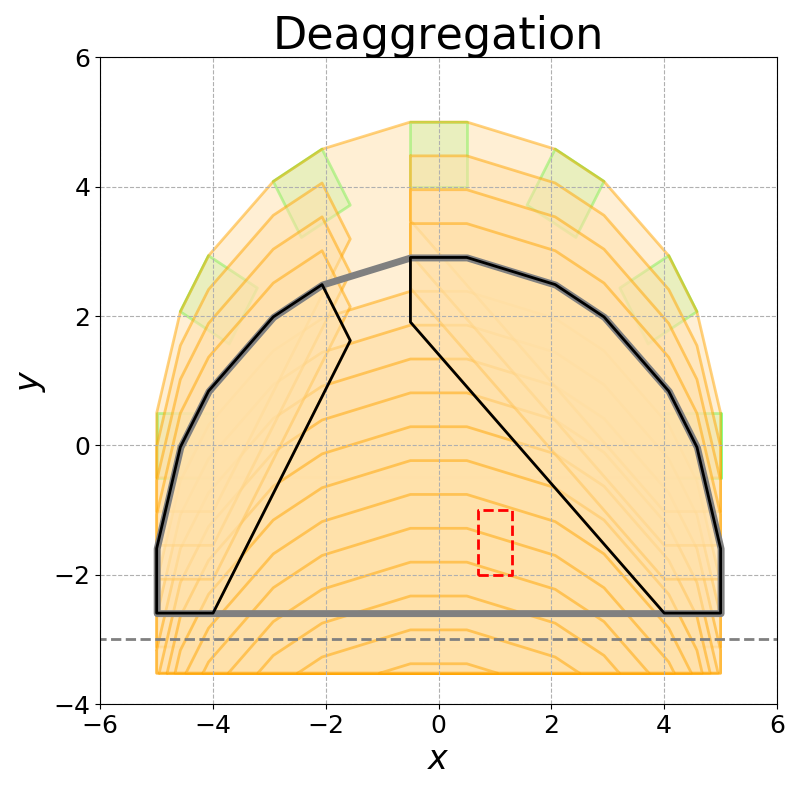
\includegraphics[width=0.7\columnwidth]{images/deagg.png}}
%\vspace{-0.4cm}
\caption{The deaggregation process is shown for a two-mode system. Upon reaching an error mode (red dotted region), the fully aggregated set of states (gray large region), is split in half (two black regions), which no longer contain error states. A video of the complete computation is available online at \url{https://gofile.io/?c=70txGD}.}
\end{figure}
%\vspace{-0.7cm}


\begin{lemma}
Algorithm~\ref{alg:aggdeagg} will return safe if and only if all the simulations starting from $\Theta$ for bounded time $k$ are safe.
\end{lemma}
\begin{proof}
This proof is a consequence of simulation equivalent reachability of Algorithm~\ref{alg:algoHybrid}. 
%
We first prove that the Algorithm~\ref{alg:aggdeagg} is sound, that is, if the algorithm returns safe, then all simulations are indeed safe and if the algorithm returns unsafe, then it is indeed unsafe. 
%
If the condition in line~\ref{ln:crucial} of Algorithm~\ref{alg:aggdeagg} is satisfied, then the reachable set $R'$ is equivalent to the one computed without any aggregation and hence is simulation equivalent. 
%
Therefore the system is indeed unsafe. 
%
Hence, whenever the algorithm returns unsafe, the system is indeed unsafe. 
%
If the algorithm returns safe, then the reachable set computed using aggregation, which is clearly an overapproximation of the reachable set, does not overlap with unsafe set. 
%
Hence, the system is safe. 


It now remains to prove that the loop in lines~\ref{ln:begLoop}-~\ref{ln:endLoop} terminates after finite number of times. 
%
This is easy to infer as there are only finitely many reachable sets that we compute. 
%
Hence, we perform only finitely many aggregations. 
%
Since we strictly do not aggregate the stars that were deaggregated before, the condition in line~\ref{ln:deagg} will only be encountered finite number of times. 
%
Hence the loop terminates and the algorithm either returns safe or unsafe.
\end{proof}


One of the advantages of generalized stars is that it allows for easy aggregation and deaggregation. 
%In the remainder of this section, we demonstrate the advantages of performing aggregation 
%
Additionally, we avoid computing the entire reachable set, but only compute the specific sections of the reachable set that are important for safety verification.
%
To keep track of the aggregations and deaggregations, we maintain a data structure called Aggregated Directed Acyclic Graph (AGGDAG).
%
%The algorithm corresponding to the aggregation and deaggregation is given in Algorithm~\ref{alg:aggdeagg}. 
%%
%A working example of the aggregation and deaggregation is provided in Figure~\ref{fig:deagg}.




%\vspace{-0.3cm}
\subsection{Aggregation of Generalized Stars}
\label{sec:aggStars}
%\vspace{-0.1cm}

In this section, we present two techniques for performing aggregation of generalized stars. The first is template based aggregation and deaggregation and the second is aggregation using convex hulls.
% advantages of using generalized stars in aggregation and deaggregation. 
%


\subsubsection{Template Based Aggregation:}
\label{sec:templateAgg}
In this paper, since all the stars we encounter have predicates that are conjunctions of linear constraints, our overapproximation is also a predicate which is a conjunction of linear constraints.

\begin{lemma}
\label{lem:agg}
Consider stars $S_1 \deq \tup{a, G, P_1}$, $S_2 \deq \tup{a, G, P_2}$, $\ldots$, $S_m \deq \tup{a, G, P_m}$ where the anchor and generators for all the stars is the same.
%
A star $S' \deq \tup{a, G, P'}$ is an overapproximation of the union, i.e., $S_1 \cup S_2 \cup \ldots \cup S_m \subseteq S'$, if and only if $(P_1 \vee P_2 \vee \ldots \vee P_k) \Rightarrow P'$.
\end{lemma}
%\begin{proof}
%Trivially follows from the definition of generalized stars.
%\end{proof}

 For computing the predicate $P'$, we use a template based method.
%
% To compute the predicate $P'$, we perform a template based method. 
%
For each location, a set of template directions $c_1^{T}, c_2^{T}, \ldots, c_{l}^{T}$ are provided by the user and the predicate $P'$ is determined by selecting the appropriate values of $d_1, d_2, \ldots, d_l$ such that the condition $(P_1 \vee P_2 \vee \ldots \vee P_k) \Rightarrow P'$ is satisfied where $P' \deq (c_1^{T}\alpha \leq d_1) \wedge (c_2^{T}\alpha \leq d_2) \wedge \ldots \wedge (c_l^{T}\alpha \leq d_l)$. 

For computing $d_j$, $1 \leq j \leq l$, we solve $m$ linear programming problems. $d_j^i$ is the maximum value of $c_j^T \alpha$ in $P_i$. That is, $d_j^1 = \mathsf{max}~ c_j^T \alpha~ \mathsf{given} P_1(\alpha) = \top$. Similarly, $d_j^2 = ~~\mathsf{max}~~ c_j^T \alpha~~ \mathsf{given} P_2(\alpha) = \top$. We also compute $d_j^3, \ldots, d_j^l$. The value of $d_j = \mathsf{max} \{d_j^1, d_j^2, \ldots, d_j^l\}$.

%\vspace{-0.6cm}
\begin{algorithm}[h!]
\SetAlgoVlined
\SetKwInOut{Input}{Input}\SetKwInOut{Output}{Output}\SetKw{Return}{return}
\Input{Predicates $P_1, P_2, \ldots, P_m$, template directions $c_1^{T}, c_2^{T}, \ldots, c_l^{T}$.}
\Output{Predicate $P'$ such that $(P_1 \vee \ldots \vee P_m)\Rightarrow P'$.}
\For{each template direction $c_j^{T}$}{
    \For{each star $S_i$}{
        $d_{j}^{i} \gets \mathsf{max}~~ c_j^T \alpha ~~\mathsf{given}~~ P_i(\alpha) = \top$\;
    }
    $d_j \gets \mathsf{max}~\{d_j^1, \ldots, d_j^m\}$\;
}

{\bf return} $P' \deq (c_1^T \alpha \leq d_1) \wedge (c_2^T \alpha \leq d_2) \wedge \ldots \wedge (c_l^{T} \alpha \leq d_l)$\;
\caption{Algorithm that performs template based aggregate of stars.}
\label{alg:aggTemplate}
\end{algorithm}
%\vspace{-0.8cm}

\begin{lemma}
The predicate $P'$ returned by Algorithm~\ref{alg:aggTemplate} is such that $(P_1 \vee \ldots \vee P_l) \Rightarrow P'$.
\end{lemma}
%\vspace{-0.1cm}

Observe that we only consider aggregation of stars with the same anchor and generators. This is because of two reasons. First, the stars that we desire to aggregate correspond to the same mode. Second, as suggested in Remark~\ref{rem:hybridAlgo}, in order to decrease the number of simulations, we change the anchor and generators of the star to the anchor and generators of the corresponding mode for computing the reachable set. Hence, we perform this aggregation after the transformation of the predicate.

It is also inexpensive to perform deaggregation of the stars aggregated using template directions. 
%
Suppose that the aggregation of the stars $S_1, S_2, \ldots, S_l$ results in too conservative overapproximation. 
%
It is then desirable to perform two separate aggregations, the first aggregation is of the first half of the stars $S_1, \ldots, S_{l/2}$ and the the second aggregation corresponding to remaining half of the stars $S_{l/2+1}, \ldots, S_{l}$. 
%
For this deaggregation, one can reuse the results of the linear programs computed in Algorithm~\ref{alg:aggTemplate}.

One might worry that template based aggregation might require solving a lot of linear programs. 
%
However, by using warm start optimization, the cost of solving several linear programs on the same polytopes becomes amortized. 
%
In warm start optimization, the seed for the next iterations of simplex start from the previous solution of a linear program.
%
Hence, the simplex algorithm skips the step of finding the feasible solution and computation is only used for finding the optimal solution for the new cost function.
%
Without such cost reduction, template based overapproximation becomes very expensive. 
%
%While the presentation here has restricted itself to only stars with same center and basis vectors (for the sake of simplicity), it is easy to observe that the template based aggregation can also be extended to stars with different centers and different basis vectors.

One of the disadvantages associated with the template based overapproximation is that the order of overapproximation is dependent on the template directions that are selected. 
%
In our experience, in addition to the axis directions, we pick the template directions dependent upon the dynamics of the location. 
%
The most appropriate template directions for improving the accuracy of overapproximation is a future area of investigation.

\subsubsection{Convex Hull Aggregation:}
\label{sec:convexhullAgg}
Given stars $S_1, S_2, \ldots, S_m$, one way to perform aggregation is to compute convex hull. 
%
A widely implemented technique in Multi Parametric Toolbox (MPT)~\cite{kvasnica2004multi} for computing convex hulls of polytopes requires transforming the representation from face representation to vertex representation and vice versa. 
%
This conversion among representations can possibly takes exponential time. 
%
We avoid these exponential time operations by using the symbolic orthogonal projections~\cite{hagemann2014reachability}. 
%
We include the basic details of this convex hull operation for the sake of completeness.

%\vspace{-0.1cm}
\begin{definition}
A symbolic orthogonal projection $\O$ is given as a pair of matrices $A \in \reals^{m \times n}$ and $L \in \reals^{m \times k}$ and ${\bf a}$ is a column vector in $\reals^m$, represented as $(A, L, {\bf a})$ prepresents the set

$$
\O = \{~x \in \reals^n~|~ \exists z \in \reals^k, Ax + Lz \leq {\bf a}\}
$$ 
\end{definition}
%\vspace{-0.1cm}

If a polytope is represented as a generalized star, there are no existentially quantified free variables in it. Hence, generalized stars that represent polytopes are special cases of symbolic orthogonal projections. The convex hull of two symbolic orthogonal projections, which can be computed by merely transforming the structural representations is presented below (taken from~\cite{hagemann2014reachability}).

%\vspace{-0.1cm}
\begin{definition}
Given two symbolic orthogonal projections $\O_1 \deq (A_1, L_1, {\bf a_1})$ and $\O_2 \deq (A_2, L_2, {\bf a_2})$, the convex hull of $\O_1$ and $\O_2$ is given as a symbolic orthogonal projection $\O_3 \deq (A_3, L_3, {\bf a_3})$ where 
$$
A_3 = 
\begin{bmatrix} 
A_1 \\ 
{\bf 0} 
\end{bmatrix}, 
L_3 = 
\begin{bmatrix} 
A_1 & L_1 & {\bf 0} & {\bf a_1} \\
-A_2 & {\bf 0} & L_2 & -{\bf a_2}
\end{bmatrix},
{\bf a_3} =
\begin{bmatrix}
{\bf a_1} \\
{\bf 0}
\end{bmatrix}
$$
Where ${\bf 0}$ represents the zero matrix of the appropriate dimension. 
\end{definition}
%\vspace{-0.1cm}

The advantage of symbolic orthogonal projection over other representations is that convex hull can be computed purely syntactically. 
%
However, observe that if $\O_1$ and $\O_2$ had $n+k$ variables and $m$ constraints, then the number of constraints in $\O_3$ is $2m$ and the number of variables is $2n+2k+1$. 
%
If one desires to perform convex hull of $r$ symbolic orthogonal projections, then the number of constraints increases by $r$ fold and the number of variables also increases  $r$ fold (it is not exponential). 
%
Hence, the number of constraints and variables required to specify the polytope exponentially increases with the number of discrete transitions. This increases the cost associated with checking the safety property of all the stars in the reachable set. Additionally, the deaggregation operation cannot reuse the computations performed during aggregation.

%\vspace{-0.3cm}
\subsection{Aggregated Directed Acyclic Graph - AGGDAG}
\label{sec:aggdag}
%\vspace{-0.1cm}

When the overapproximation obtained from reachable set is too convervative and overlaps with the unsafe set, we perform deaggregation. In typical reachable set computation tools, one has to resume the computation of the reachable set from the newly deaggregated sets. However, we leverage the properties of generalized stars in reachable set computation and decrease the computations that need to be performed.

%\vspace{-0.1cm}
\begin{remark}
\label{rem:changePred}
Consider an aggregated star $S_a \deq \tup{c, V, P_a}$ and the bounded time reachable set be $S_{a_1}, \ldots, S_{a_k}$ where $S_{a_i} \deq \tup{c_i, V_i, P_a}$. After performing deaggregation, $S_a$ results in stars $S_{b}$ and $S_c$ where $S_{b} \deq \tup{c, V, P_{b}}$ and $S_{c} \deq \tup{c, V, P_{c}}$, then the reachable set starting from $S_{b}$ is given as $S_{b_1}, \ldots, S_{b_k}$ where $S_{b_i} \deq \tup{c_i, V_i, P_b}$. Similar relation holds for $S_{c}$ as initial set. Therefore, one need not recompute the center and basis vectors for computing the reachable set with new initial set. Merely changing the predicate in the generalized stars suffices.
\end{remark}
%\vspace{-0.1cm}

While recomputing the new center and basis vectors can be avoided, we also reduce our effort by checking intersection with guards and overlap with unsafe set after deaggregation. That is, when an aggregation is performed and the reachable set is computed, we only keep track of the stars that either overlap with the unsafe set or encounter a discrete transition. We keep track of the relationship between the reachable sets called as Aggregated Directed Acyclic Graph (AGGDAG).

%\vspace{-0.1cm}
\begin{definition}
\label{def:aggdag}
An AGGDAG is a directed graph $(G, H)$ where, the set of nodes $G$ corresponds to the generalized stars obtained during the reachable set computation that encounter the discrete transitions or overlap with the unsafe set, and the set of edges $E$ represents the successor relationship among these generalized stars.
\end{definition}
%\vspace{-0.4cm}

%\vspace{-0.3cm}
\begin{figure}
\centering
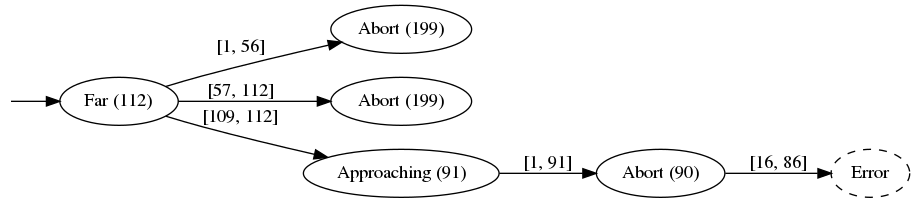
\includegraphics[width=0.9\textwidth]{images/viz2}
\caption{Example of an aggdag.}
\label{fig:aggdagex1}
\end{figure}
%\vspace{-0.5cm}

%\vspace{-0.3cm}
\begin{example}
Figure~\ref{fig:aggdagex1} is an example of aggdag where the hybrid automata has 3 modes of operation, namely, {\em Far}, {\em Approaching}, and {\em Abort}. The initial set starting from the Far mode takes the discrete transitions to Abort in the time duration $[1,56]$ and $[57,112]$ and stays in the Abort mode without encountering any unsafe set. The successors of the stars that encounter a discrete transition to the Approaching mode in the time interval $[109,112]$, encounter the unsafe set in future. In the Figure~\ref{fig:aggdagex1}, the star representing the node Approaching is the collection of the stars that encounter the discrete transition in the time interval $[109, 112]$. Simiarly, the node Abort [Abort (90) to be more precise] corresponds to the collection of the stars that take the discrete transition from Approaching mode to the Abort mode. Out of the stars in the Abort(90) node, the violation of safety propery happens between the time intervals $[16,86]$.
\end{example}

To check if the safety property is indeed violated in the reachable set computation, we first inspect the aggdag in Figure~\ref{fig:aggdagex1}. Since the safety is violated in trajectories in Abort mode, we need to inspect whether there is overapproximation induced in the aggregation of the reachable set in the path from the root node to the Abort node. 
This overapproximation can be at two instances, first, the aggregation of stars in the Approaching modes in the interval $[109, 112]$ or second, in the Abort mode in the interval $[1,91]$.  If both these reachable set do not have any aggregation, then we have proof that the overlap with the unsafe set is indeed a safety violation. Hence, refining only the aggregation associated with the reachable sets in the specific interval of time suffices.


The aggdag is useful only in bookkeeping the states that encounter the discrete transitions. The strategy for deaggregation is still decided by the user. In our tool, we have implemented two deaggregation strategies, first, from the leaf to root and second, from root to leaf. In the case of leaf to root, we first deaggregate the reachable sets that are closest to the safety violation and continue the deaggregation to the top. In Figure~\ref{fig:aggdagex1}, in the leaf to root strategy, we would first deaggregate the states taking the discrete transition from Approaching to Abort. In the root to leaf strategy, the deaggregation is performed at the node closest to the root node in the path leading to the unsafe overlap. In Figure~\ref{fig:aggdagex1}, under the root to leaf strategy, one would deaggregate the stars in the discrete transition from Far to Approaching. The best deaggregation strategy for proving safety or discovering the counterexample is still an area to be investigated and is a part of future research.







\section{Case Study: Spacecraft Rendezvous Passive Safety}
\label{sec:casestudy}

We evaluate our method on a spacecraft rendezvous passive safety case study. The system consists of a primary chaser spacecraft moving towards a secondary, free-flying object (such as a satellite) and performing close-proximity maneuvers.
%
The maneuver is analyzed in relative coordinates, as shown in Figure~\ref{fig:chaser}.
%
The verification goal is to ensure \emph{passive safety}: at any time in the maneuver, a system failure may occur and the resulting propulsion-free trajectory must avoid colliding with the target satellite.
%
This requirement comes from real-world failures. In 2005, NASA’s DART spacecraft was intended to rendezvous with the MUBLCOM satellite, but due to depleted propellant instead collided with the target satellite (a loss of a
\$110 million project)~\cite{croomes2006overview}.

\begin{figure}[t]
\centerline{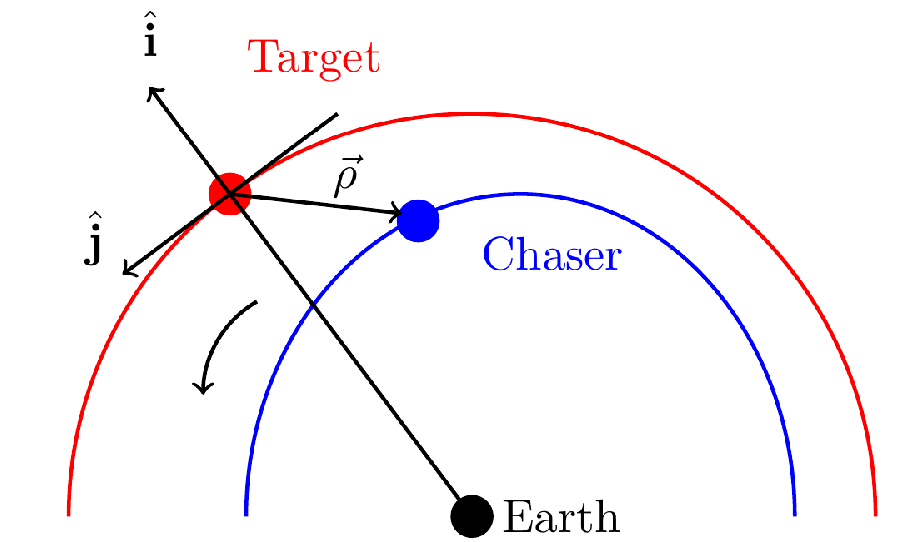
\includegraphics[width=0.5\columnwidth]{images/chaser.png}}
\caption{Collisions are checked between spacecraft in orbit in relative coordinates (image from~\cite{chan2017verifying}).}
\label{fig:chaser}
\end{figure}

Our model is based on a published benchmark for this system~\cite{chan2017verifying,jewison2016spacecraft}. The system is modeled as a hybrid automaton with different discrete modes depending on the sensors being used for navigation, and an LQR controller is designed to meet physical and geometric safety constraints.
%
The relative dynamics are linearized using the Clohessy-Wiltshire-Hill (CWH) equations~\cite{wh1960terminal}, which is often used in close proximity operations. The hybrid automaton consists of three modes, two for different navigation strategies, and one for the passive dynamics, shown in Figure~\ref{fig:ha}.
%
In our analysis, we check for passive safety over the full time bound, $t1=0$ and $t_2=200$.
%
We focus on the collision-free safety property that the spacecraft must remain 0.2 meters apart at all times.

\begin{figure}[t]
\centerline{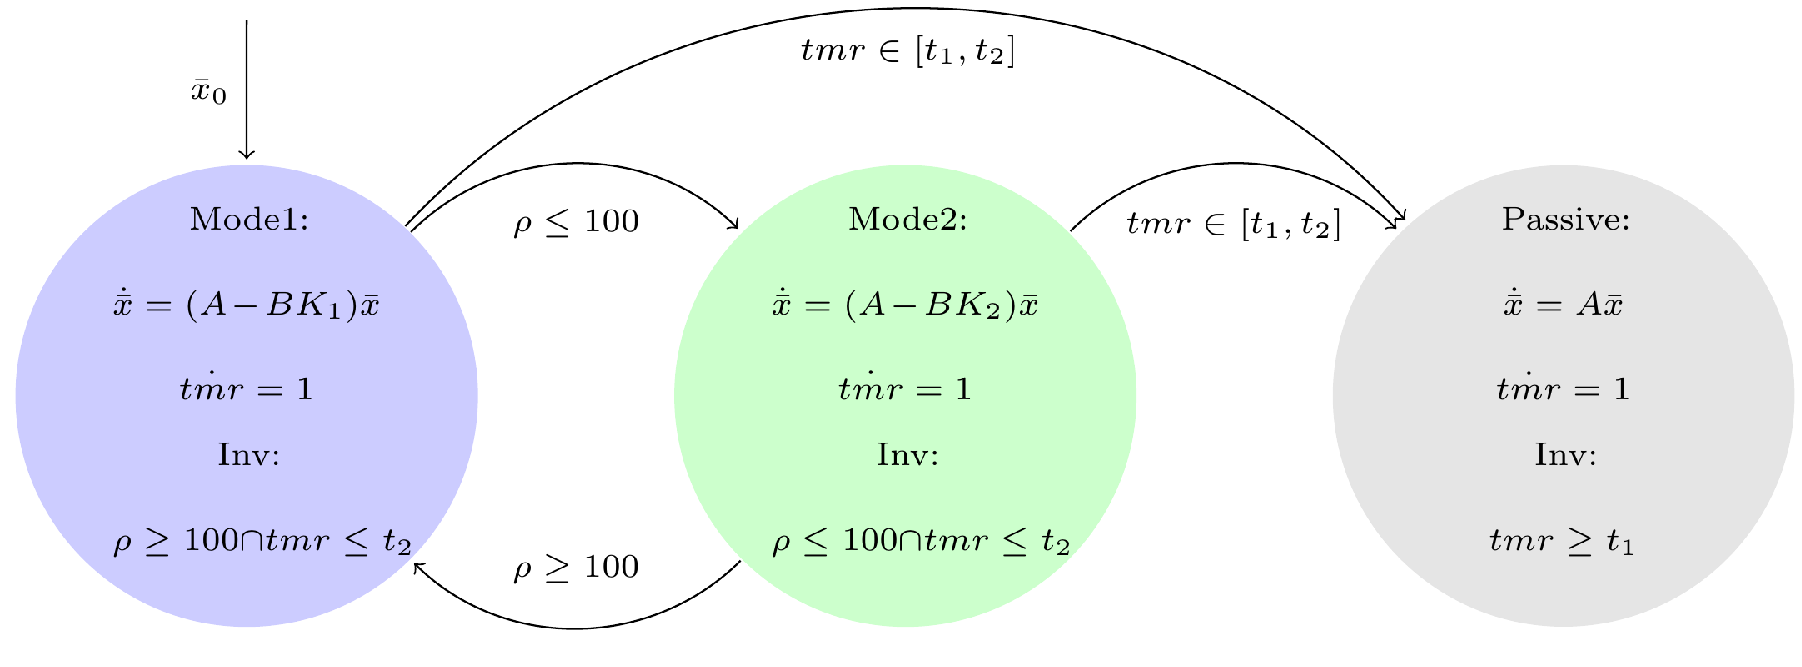
\includegraphics[width=0.9\columnwidth]{images/ha.png}}
\caption{Hybrid automaton model of case study (image from~\cite{chan2017verifying}). We check for passive safety over the full time bound ($t_1=0$ and $t_2=200$).}
\label{fig:ha}
\end{figure}

Although several tools have successfully analyzed a version of this model in the ARCH hybrid systems tools competition in 2018~\cite{archcomp18linear}, a critical simplification was made: the competition model did not actually check the passive safety requirement. In particular, the competition model used a \emph{fixed} time to transition to the passive model. This is an unrealistic simplification, since the time of failure cannot not be known in advance. 

The analysis done in the original work~\cite{chan2017verifying} is slightly better, in that it checks for passive safety for a known 5 minute failure interval during the 200 minute maneuver. The reason stated in the paper for this is that, if larger time intervals are used,
``the initial set of states under the Passive mode is large, making it very difficult to prove safety.'' The suggestion is then to create subintervals that cover the full time range of transitions to the passive mode, and then run several experiments. Presumably, a manual guess-and-check approach should be used to create these subintervals.

The full passive safety problem can be solved using the proposed aggdag method. Our aggdag method performs full state aggregation (an overapproximation), and then recursively desegregates if the overapproximation reaches an error mode. The advantage of this is that (1) the method is fully automatic, (2) steps where the overapproximation is safe can be skipped by the refined sets, which is more efficient than using multiple independent experiments, and (3) if an error exists, it will be detected after full deaggregation is performed, which allows the generation of a concrete counter example trace. Other verification tools for linear hybrid systems do not typically generate counter-examples when safety cannot be proven.

Our experiments are performed on a system with an Intel i5-5300U CPU running at 2.30GHz with 16GB RAM and using Ubuntu Linux 18.04.
%
We first analyze the runtime of the method, shown in Table~\ref{tab:runtime}.
%
We look at the number of seconds and the number of reachability steps needed to prove safety for the system as we vary the step size.
%
A reachability step is a single continuous post operator, or a refinement step when performing deaggregation.
%
As the step size for this system is reduced, the number of combinations of steps that reach each guard in the hybrid automaton increases.
%
However, from the table, we observe that the runtime and number of steps remains inversely proportional to the step size.
%
This means that the analysis is successfully using state set aggregation to eliminate combinatorial explosion, with sufficient
precision to guarantee the system avoid collisions.

\setlength{\tabcolsep}{2pt}
\begin{table}[t]
\caption{Safe maneuver check time.}
\label{tab:runtime}
\centering
\setlength{\aboverulesep}{0.0pt}
\setlength{\belowrulesep}{0.0pt}
\setlength{\extrarowheight}{-0.2ex}
\begin{tabular}{@{}lll@{}}
  \toprule
  Step Size & Runtime & Num Steps \\
  \midrule
  1.0 & 5.1 & 726 \\
  0.5 & 11.0 & 1508 \\
  0.2 & 34.7 & 4657 \\
  0.1 & 73.2 & 9557 \\
\bottomrule
\end{tabular}
\end{table}

The analysis is exact, in that if the system were to have a collision, the deaggregation approach would eventually find it.
%
In the next experiment, we increase the collision distance from 0.2 to 1.0 meters.
%
In this case, a collision is possible, and our approach generates the corresponding counter-example trace (initial state and switching times)
for every step size analyzed.
%
The results are shown in Table~\ref{tab:runtime_unsafe}.
%
The runtime increases compared with the safe version of the benchmark, as more deaggregation is necessary in this case since a real error trace is
present (the deaggregation continues until single time instants are considered, at which point a concrete trace can be generated).

\setlength{\tabcolsep}{2pt}
\begin{table}[t]
\caption{Unsafe maneuver check time.}
\label{tab:runtime_unsafe}
\centering
\setlength{\aboverulesep}{0.0pt}
\setlength{\belowrulesep}{0.0pt}
\setlength{\extrarowheight}{.0ex}
\begin{tabular}{@{}lll@{}}
  \toprule
  Step Size & Runtime & Num Steps \\
  \midrule
  1.0 & 9.2 & 1232 \\
  0.5 & 34.8 & 3736 \\
  0.2 & 94.7 & 10958 \\
  0.1 & 243 & 25091 \\
\bottomrule
\end{tabular}
\end{table}

Overall, our main evaluation result is that analysis of this system is possible though maintaining the aggdag data structure  and
performing deaggregation upon reaching an error mode.
%
Prior to this, all analysis on this model checked for switching to the passive mode at a single time instant or small time window, since otherwise the methods would have too much error to prove the system is safe.
%
For this reason, we could not perform a tool runtime comparison; analysis is not possible on this model with existing tools.
%
Furthermore, we were able to generate counterexamples in the cases where the safety property was violated.


%\vspace{-0.2cm}
\section{Conclusions}
%\vspace{-0.4cm}
In this paper we have focused on computing accurate reachable set computation of hybrid automata where there is high nondeterminism in the discrete transitions. We presented two common techniques used for aggregation and highlighted the relative merits and demerits of each technique. We also presented AGGDAG data structure and outlined the deaggregation strategies that were implemented. Using the techniques we were able to handle the challenging case studies of satellite rendezvous mission and gearbox meshing.

Handling discrete transitions is still a major hurdle in scalable and accurate computation of reachable set for linear hybrid systems. As a part of future work, we intend to explore intelligent aggregation and deaggregation strategies that adapt based on the dynamics to provide an accurate reachable set.

\section*{Acknowledgements} The work done in this paper is based upon work supported by the National Science Foundation (NSF) under grant numbers CNS 1739936, 1935724. Any opinions, findings, and conclusions or recommendations expressed in this publication are those ofthe authors and do not necessarily reflect the views of NSF.
%
Effort sponsored in whole or in part by the Air Force Research Laboratory, USAF, under Memorandum of Understanding/Partnership Intermediary Agreement No. 
FA8650-18-3-9325 and prime contract FA8650-15-D-2516.  The U.S. Government is authorized to reproduce and distribute reprints for Government purposes notwithstanding any copyright notation thereon. The views and conclusions contained herein are those of the authors and should not be interpreted as necessarily representing the official policies or endorsements, either expressed or implied, of the Air Force Research Laboratory.


\vspace{-0.2cm}
\bibliographystyle{ACM-Reference-Format}
\bibliography{bibfile}


\end{document}
